\documentclass[aspectratio=169]{beamer}
 
\usepackage[utf8]{inputenc}
\usepackage{lipsum}

\usepackage[backend=biber,bibencoding=utf8,style=verbose-inote,citestyle=authoryear]{biblatex}
\bibliography{references}

%%%%%%%%%%%%%%%%%%%%%%%%%%%%%%%%%%%%%%%%%%%%%%%%
% Set Helvetica Font in Text and Math in LaTeX %
%%%%%%%%%%%%%%%%%%%%%%%%%%%%%%%%%%%%%%%%%%%%%%%%
\usepackage[helvet]{sfmath}
\usepackage[scaled=1]{helvet}
\usepackage[T1]{fontenc}
\renewcommand\familydefault{\sfdefault} 
\everymath={\sf}
\usepackage{fontspec}

\usepackage{subcaption}

\hypersetup{
    colorlinks=true,
    linkcolor=blue,
    filecolor=magenta,      
    urlcolor=cyan,
    pdftitle={Overleaf Example},
%    pdfpagemode=FullScreen,
}

\usepackage{hyperref}
\hypersetup{
    colorlinks = false,
    linkbordercolor = {white}
}


% use settings files
\usetheme[progressbar=frametitle]{metropolis}

%%%%%%%%%%%%%%%%%%%%%%%%%%%%%%%%%%%%%%%%%%%%%%%%%%%%%%%%%%%%%%%%
% Color settings
\definecolor{ru_white}{HTML}{FFFFFF}
\definecolor{ru_red}{HTML}{ed1c24}
\definecolor{black}{HTML}{000000}
\definecolor{gray}{HTML}{A9A9A9}
\definecolor{light_gray}{HTML}{E0E0E0}
\setbeamercolor{frametitle}
{
  use=palette primary,
  parent=palette primary,
  fg = ru_white,
  bg = ru_red
}
% fg means "foreground" and bg means "background"
\setbeamercolor{title separator}{ fg=ru_red }
\setbeamercolor{section bar}{ fg=ru_red, bg=ru_red }
\setbeamercolor{progress bar in section page}{
%   use=progress bar,
%   parent=progress bar
    fg=black,
    bg=ru_red
}

\setbeamercolor{normal text}{%
  fg=black,
  bg=white
}
\setbeamercolor{alerted text}{%
  fg=ru_red,
}
\setbeamercolor{example text}{%
  fg=black,
}

\setbeamercolor{progress bar in head/foot}{ fg=black, bg=gray } % use this line to enable the progress bar
% \setbeamercolor{progress bar in head/foot}{ fg=black, bg=black } % use this line to have a divider instead of a progress bar

% \setbeamertemplate{frame numbering}{} % uncomment this line to remove slide numbers
\titlegraphic{\hfill
\includegraphics[height=2.0cm]{images/HR_logo_hringur_hires}}
%\logo{
\includegraphics[width=.1\textwidth]{images/HR_logo_hringur_lowres}\vspace{-0.05\paperwidth}\hspace*{.04\paperwidth}} % uncomment this line to include the RU logo on each slide
\logo{
\includegraphics[width=.1\textwidth]{images/HR_logo_hringur_lowres}\vspace{-0.05\paperwidth}\hspace*{0.5\paperwidth}} % uncomment this line to include the RU logo on each slide

\setbeamertemplate{itemize items}[default]

\setbeamerfont{bibliography entry author}{size=\tiny,series=\normalfont}
\setbeamerfont{bibliography entry title}{size=\tiny,series=\bfseries}
\setbeamerfont{bibliography entry location}{size=\tiny,series=\normalfont}
\setbeamerfont{bibliography entry note}{size=\tiny,series=\normalfont}

\makeatletter
\setlength{\metropolis@progressinheadfoot@linewidth}{1pt}               % thickness of progress bar on normal pages
\setlength{\metropolis@titleseparator@linewidth}{0.5pt}                 % thickness of separator on title page
\setlength{\metropolis@progressonsectionpage@linewidth}{0.5pt}          % thickness of progress bar on section page


\setbeamertemplate{frametitle}{%
    \vspace*{-0.12cm}
     \begin{beamercolorbox}[wd=\paperwidth,ht=2ex,dp=0.8ex,left]{frametitle}%
    %   \hspace*{2ex}\insertframetitle%
        % \vspace*{\fill}
        \hspace*{2ex}\insertframetitle%
        % \vspace*{\fill}
     \end{beamercolorbox}}

\usepackage{ifxetex,ifluatex}

\usepackage{tikz}
\usepackage{framed}

% conditional for xetex or luatex
% \newif\ifxetexorluatex
% \ifxetex
%   \xetexorluatextrue
% \else
%   \ifluatex
%     \xetexorluatextrue
%   \else
%     \xetexorluatexfalse
%   \fi
% \fi

% \ifxetexorluatex
%   \usepackage{libertine} % or use \setmainfont to choose any font on your system
%   \newfontfamily[Ligatures=TeX]{Linux Libertine O} % selects Libertine as the quote font
% \else
%   \usepackage{libertine} % or any other font package
%   \newcommand* {\fontfamily{LinuxLibertineT-LF}} % selects Libertine as the quote font
% \fi

\newcommand*\quotesize{60} % if quote size changes, need a way to make shifts relative
% Make commands for the quotes
\newcommand*{\openquote}
   {\tikz[remember picture,overlay,xshift=-4ex,yshift=-2.5ex]
   \node (OQ) { \fontsize{\quotesize}{\quotesize}\selectfont``};\kern0pt}

\newcommand*{\closequote}[1]
  {\tikz[remember picture,overlay,xshift=4ex,yshift={#1}]
   \node (CQ) { \fontsize{\quotesize}{\quotesize}\selectfont''};}

% select a colour for the shading
\definecolor{shade_color}{HTML}{F8F8F8}
\colorlet{shadecolor}{light_gray}

\newcommand*\shadedauthorformat{\emph} % define format for the author argument

% Now a command to allow left, right and centre alignment of the author
\newcommand*\authoralign[1]{%
  \if#1l
    \def\authorfill{}\def\quotefill{\hfill}
  \else
    \if#1r
      \def\authorfill{\hfill}\def\quotefill{}
    \else
      \if#1c
        \gdef\authorfill{\hfill}\def\quotefill{\hfill}
      \else\typeout{Invalid option}
      \fi
    \fi
  \fi}
% wrap everything in its own environment which takes one argument (author) and one optional argument
% specifying the alignment [l, r or c]
%
\newenvironment{shadequote}[2][l]%
{\authoralign{#1}
\ifblank{#2}
   {\def\shadequoteauthor{}\def\yshift{-2ex}\def\quotefill{\hfill}}
   {\def\shadequoteauthor{\par\authorfill\shadedauthorformat{#2}}\def\yshift{2ex}}
\begin{snugshade}\begin{quote}\openquote}
{\shadequoteauthor\quotefill\closequote{\yshift}\end{quote}\end{snugshade}}

% Other packages
\usepackage{enumitem}
\setitemize{label=\usebeamerfont*{itemize item}%
  \usebeamercolor[fg]{itemize item}
  \usebeamertemplate{itemize item}}

\usepackage{amssymb}
\newcommand*{\QEDA}{\hfill\ensuremath{\blacksquare}}

\usepackage{datetime}
\newdateformat{specialdate}{\twodigit{\THEDAY} \ \monthname[\THEMONTH] \THEYEAR}

%%%%%%%%%%%%%%%%%%%%%%%%%%%%%%%%%%%%%%%%%%%%%%%%%%%%%%%%%%%%%%%%%

\newcommand{\nologo}{\setbeamertemplate{logo}{}}
\newcommand{\yeslogo}{\logo{\vspace{-0.5cm}
\includegraphics[width=1.5cm]{./images/HR_logo_hringur_lowres}\hspace{0.5cm}}}

\yeslogo

\newif\ifpause
\pausetrue
%\pausefalse
\newcommand{\mypause}{\ifpause \pause \fi}

%Information to be included in the title page:
\title{Autonomous Multirotor Landing on Landing Pads\\and Lava Flows}
\author{Joshua Springer}
\institute{Reykjavik University\\Department of Computer Science\\Supervisor: Marcel Kyas}

\date{7 December 2022}

\begin{document}

\maketitle

\nologo

\begin{frame}{Topic Overview}
	\begin{itemize}
		\item Autonomous drone landing: hard, needs to be precise
		\item Often depends on GPS, blind to obstacles
		\item Often needs to be more precise than GPS (or GPS-denied)
		\item Landing pads: fiducial markers
		\item Terrain analysis
		\item Aesthetics:
		\begin{itemize}
			\item GPS-independent
			\item Embedded processing only $\rightarrow$ efficient, quick, dedicated hardware
			\item No active ground infrastructure (e.g.~ground stations with telemetry, computing hardware)
			\item Prefer passive sensors (e.g.~RGBD cameras instead of LIDAR/RADAR)
		\end{itemize}
	\end{itemize}
\end{frame}

\section{Structured Case: Landing Pads}

\begin{frame}{Fiducial Markers}
\begin{columns}
\begin{column}{0.4\textwidth}
	\centering
	\begin{tabular}{cc}
		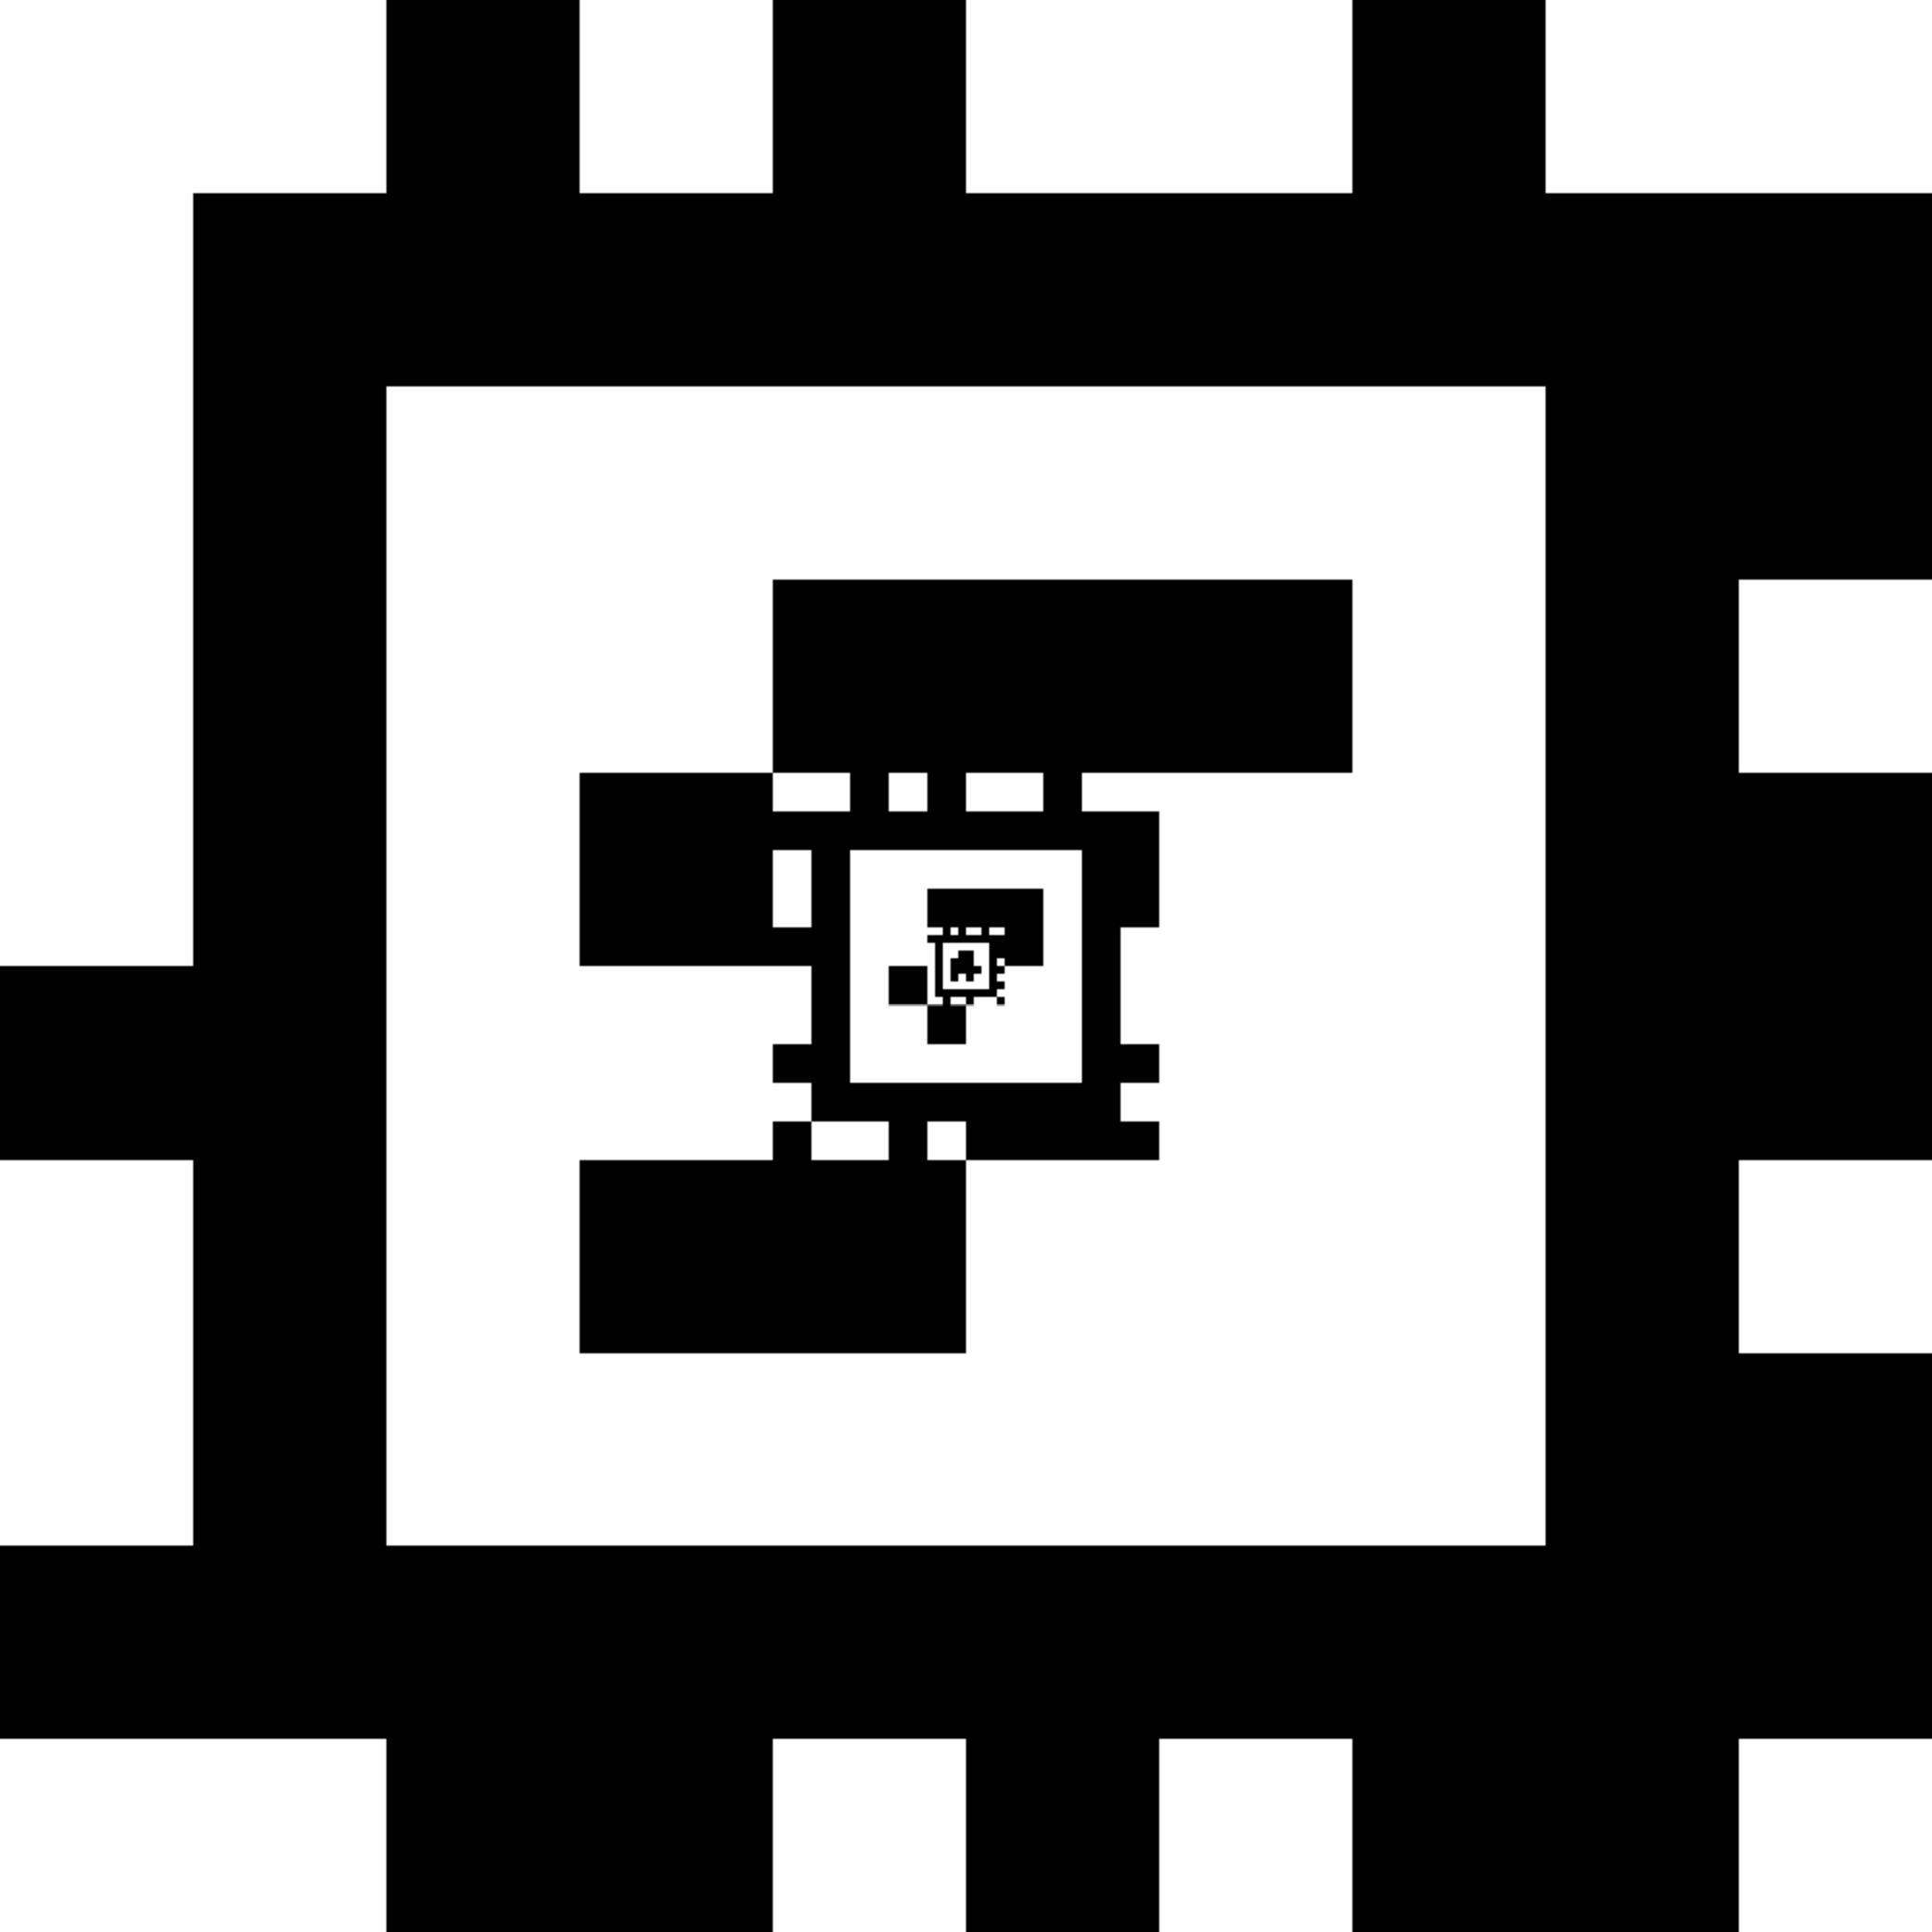
\includegraphics[width=2cm]{./images/tagCustom48h12_00002_00001_00000}
		&
		\includegraphics[width=2cm]{./images/tagCustom24h10_00002_00001_00000}
		\\
		April Tag 48h12%\footnotemark%~\footcite{apriltag3_paper}
		\footnote[frame]{\cite{apriltag3_paper}}
		&
		April Tag 24h10%~\footcite{fiducial_precursor_evaluation}
		\\
		
\includegraphics[width=2cm]{./images/whycode_20_8}
		&
		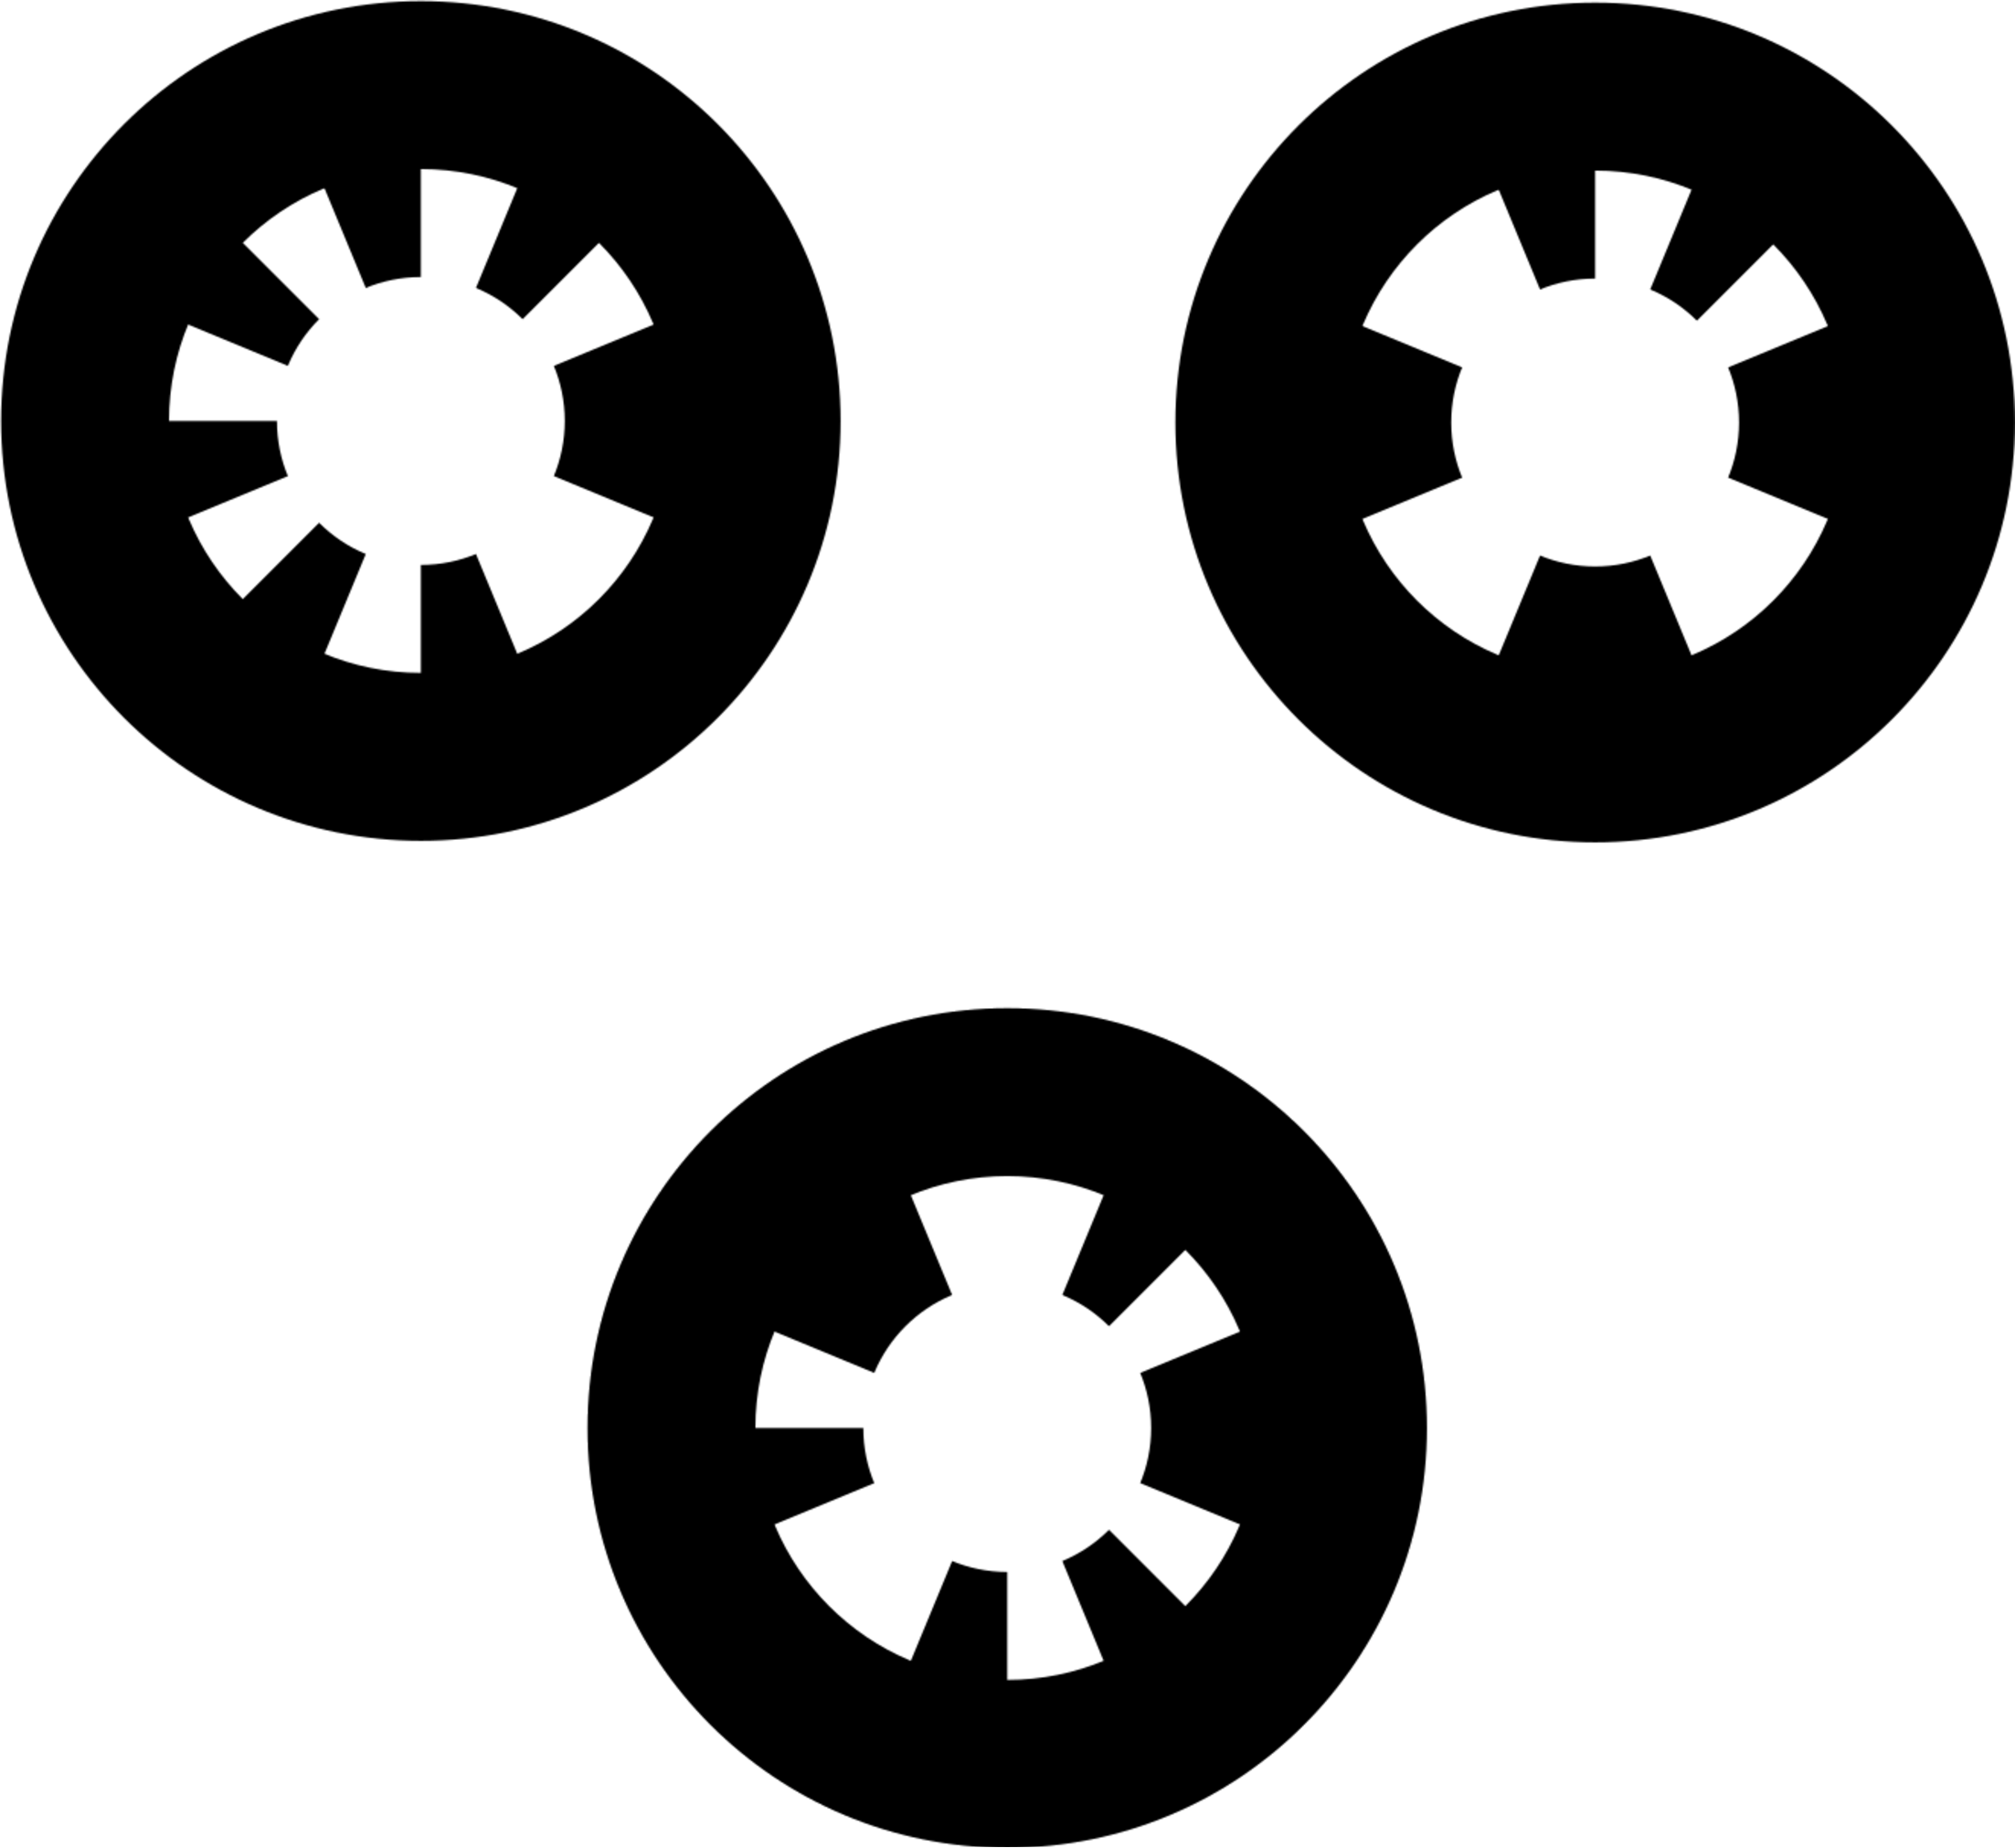
\includegraphics[width=2cm]{./images/whycode_multi}
		\\
		WhyCode (Orig)%\footnotemark%~\footcite{whycode_paper}
		\footnote[frame]{\cite{whycode_paper}}
		&
		WhyCode Multi%~\footcite{fiducial_precursor_evaluation}
	\end{tabular}
\end{column}
\begin{column}{0.6\textwidth}
	\centering
	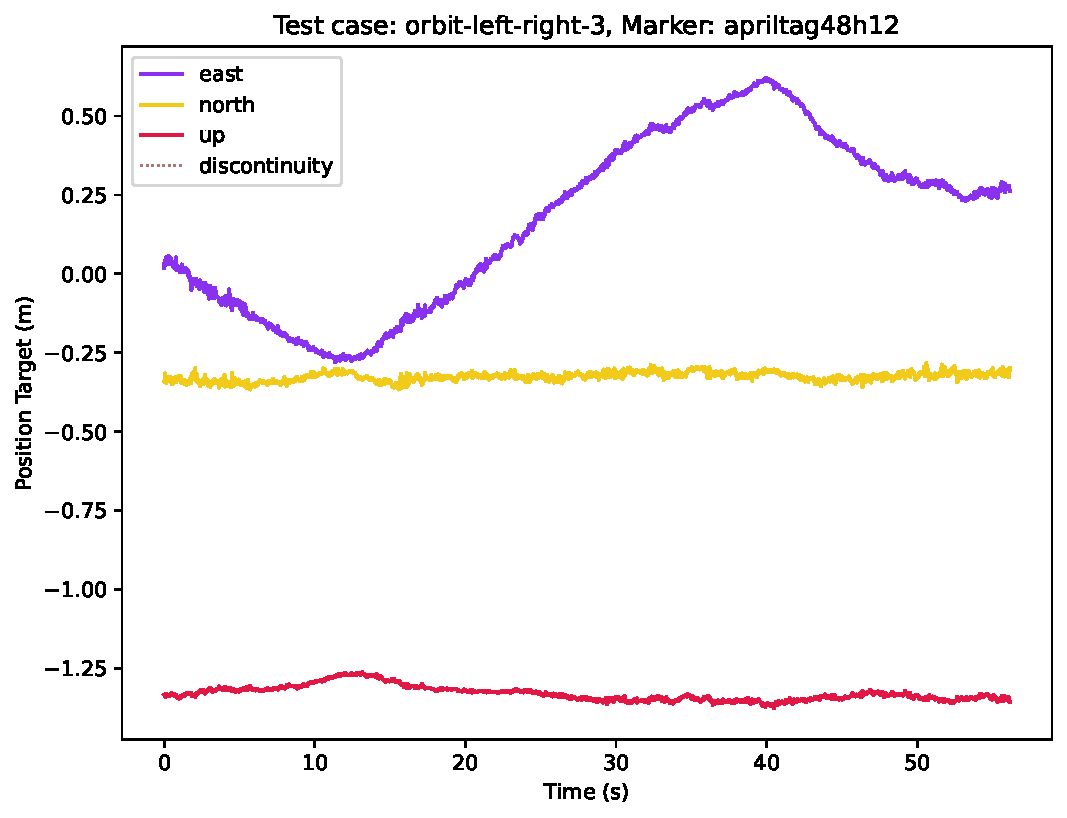
\includegraphics[width=\linewidth]{images/orbit-left-right-3_apriltag48h12_position-target}
\end{column}
\end{columns}
%		\footcitetext{apriltag3_paper}
%		\footcitetext{whycode_paper}
\end{frame}
%\begin{frame}{Fiducial Markers}
%\begin{columns}
%\begin{column}{0.4\textwidth}
%	\centering
%	\begin{tabular}{cc}
%		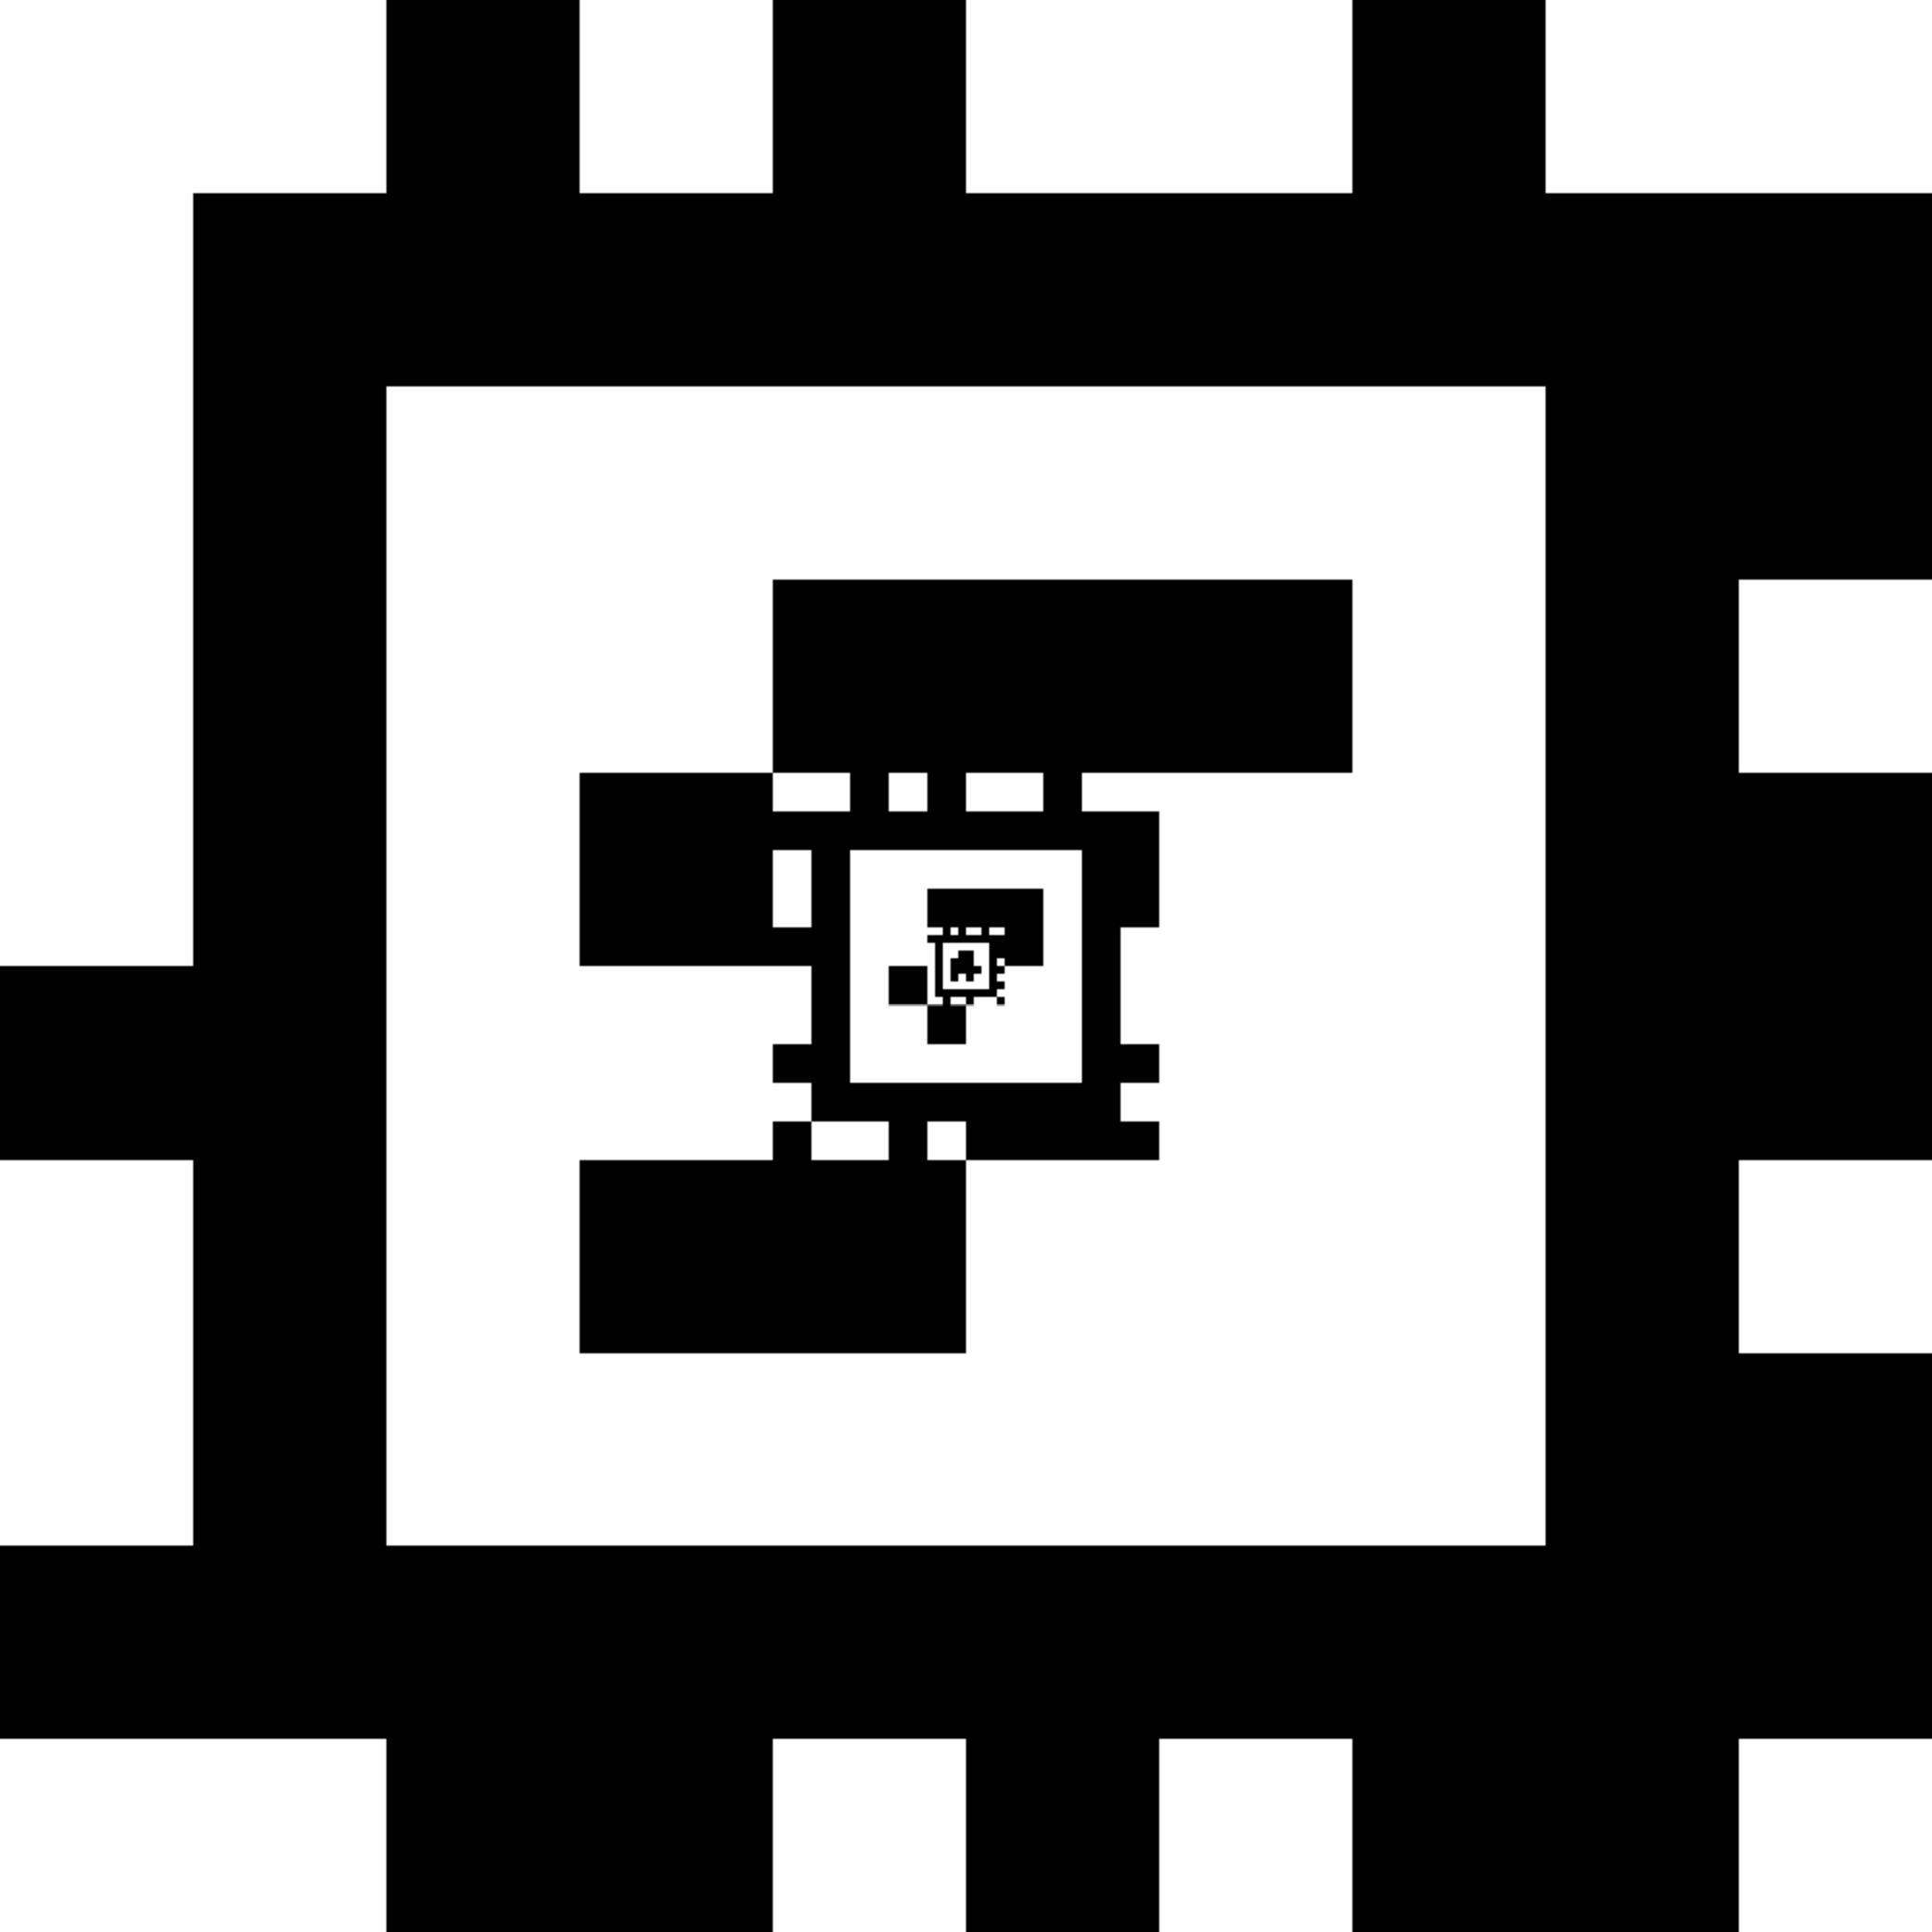
\includegraphics[width=2cm]{./images/tagCustom48h12_00002_00001_00000}
%		&
%		\includegraphics[width=2cm]{./images/tagCustom24h10_00002_00001_00000}
%		\\
%		April Tag 48h12~\footcite{apriltag3_paper}
%		&
%		April Tag 24h10%~\footcite{fiducial_precursor_evaluation}
%		\\
%		
\includegraphics[width=2cm]{./images/whycode_20_8}
%		&
%		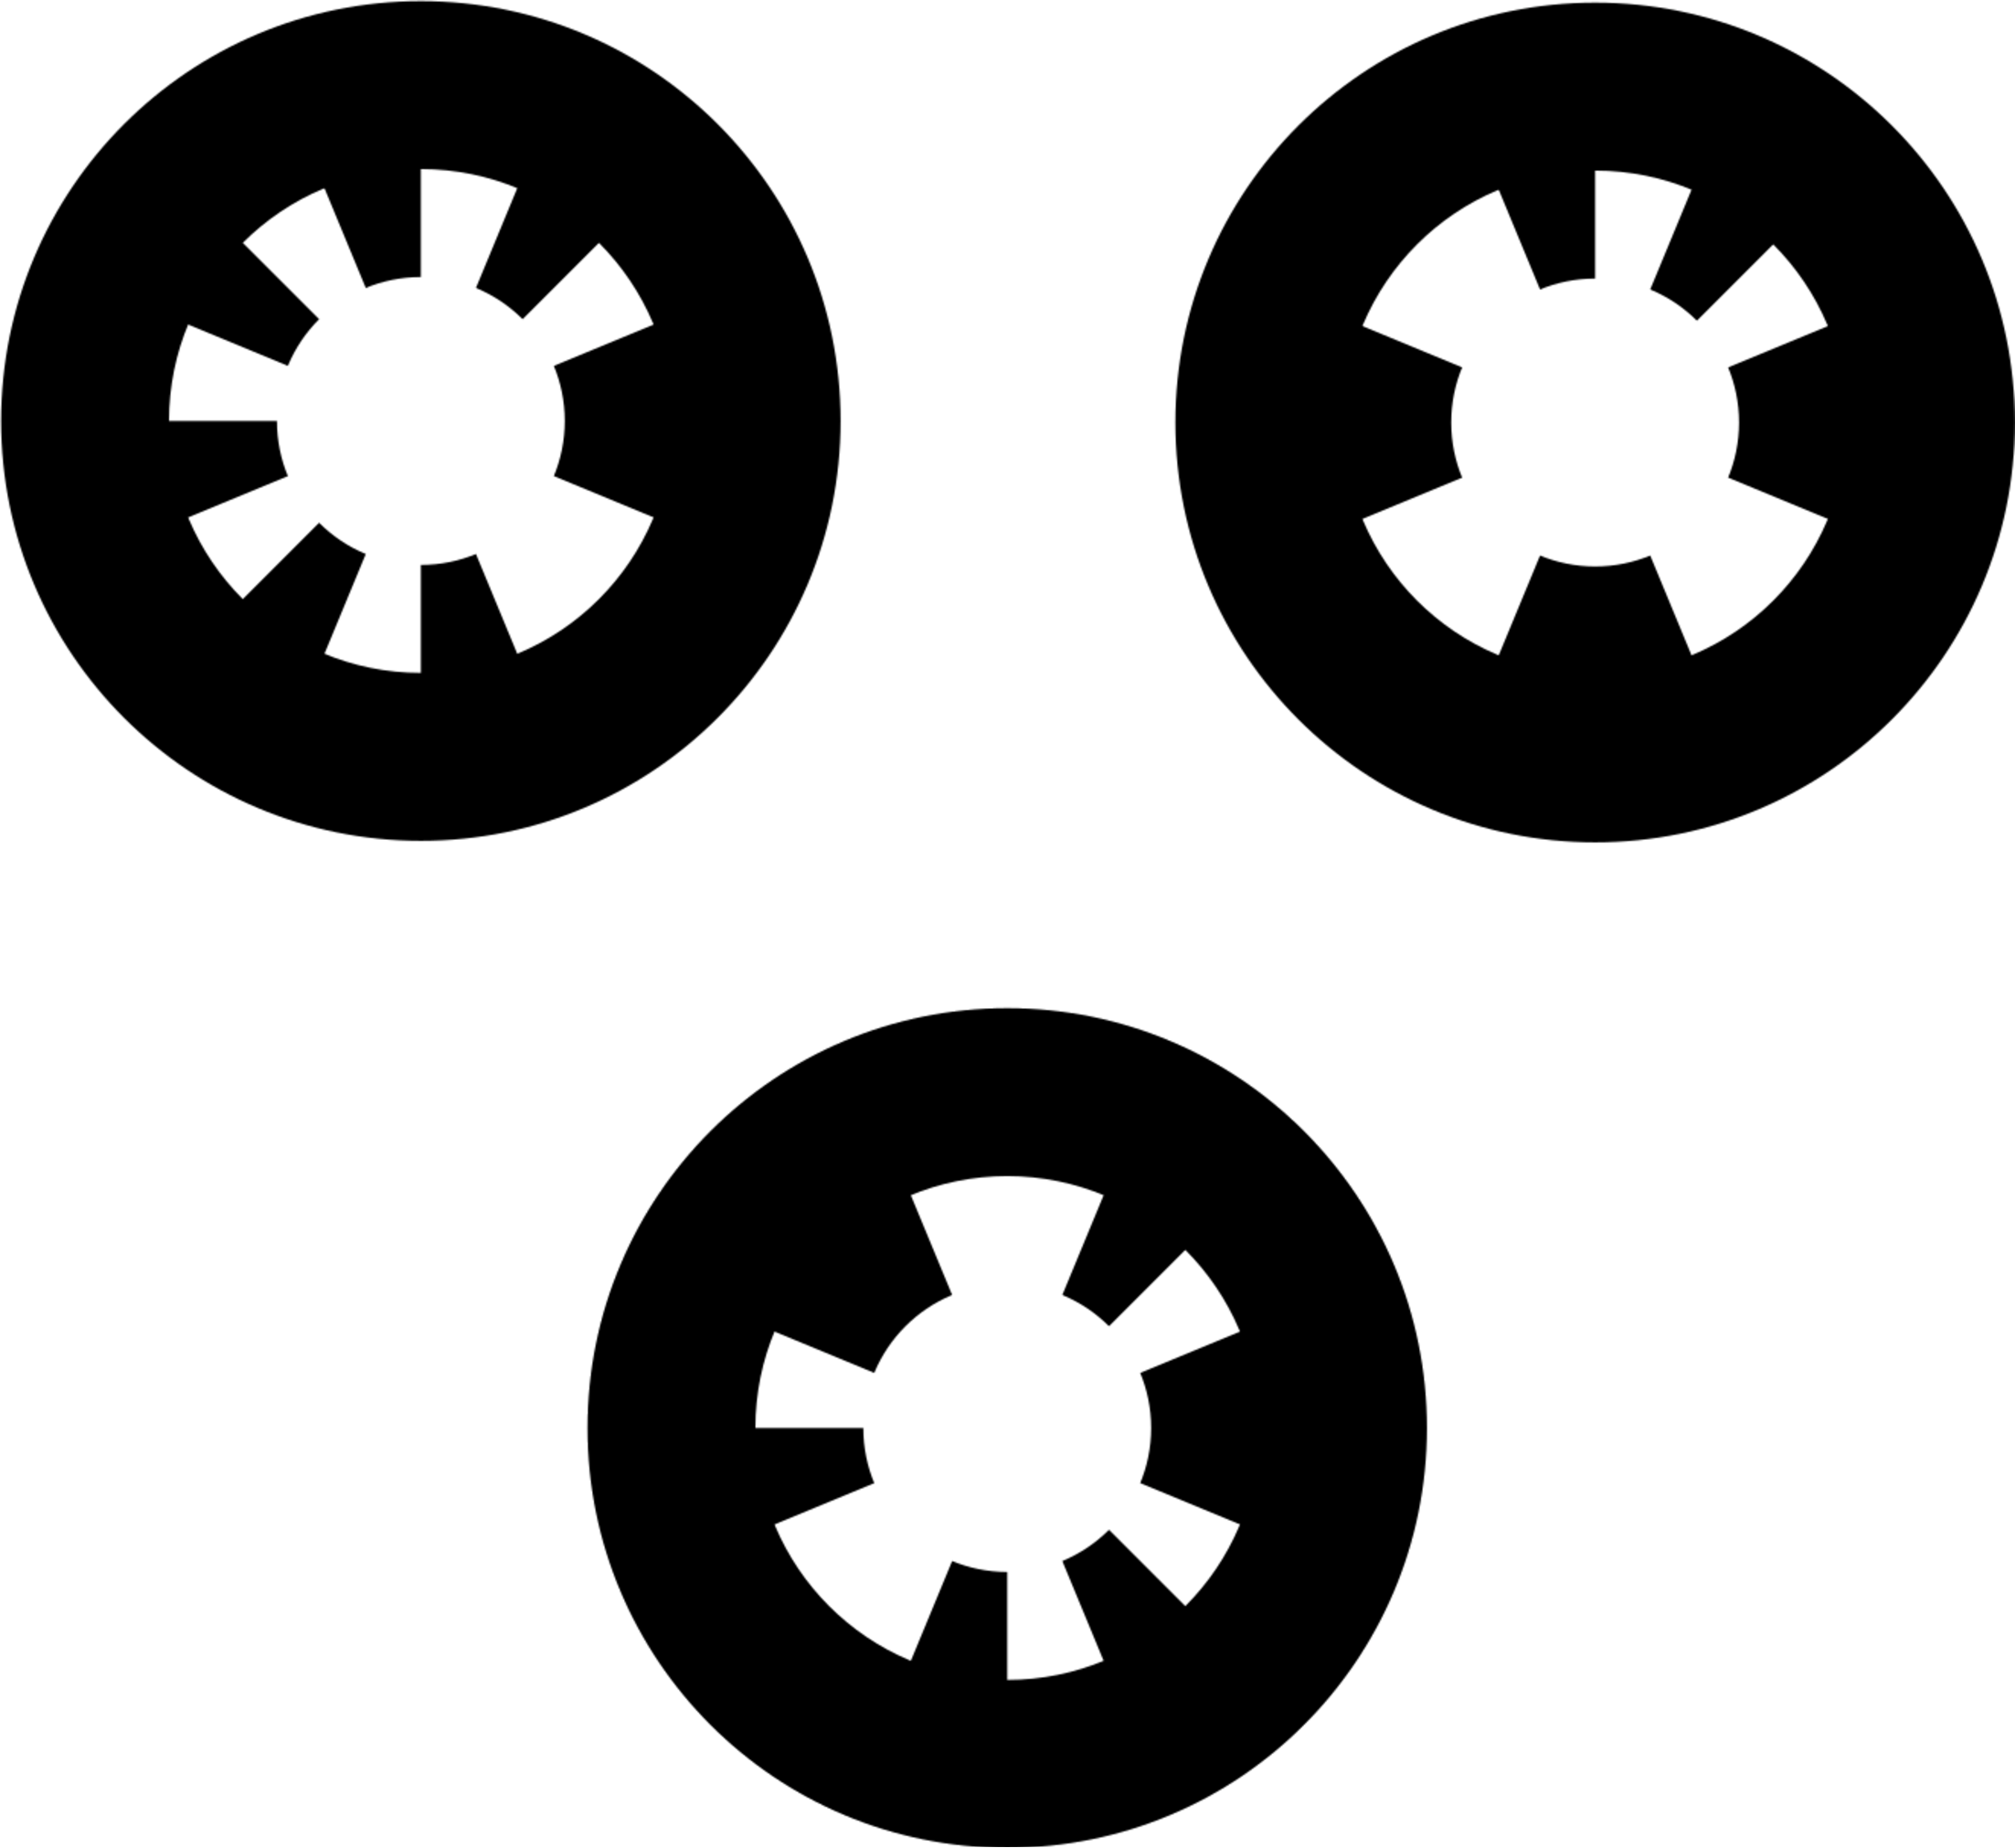
\includegraphics[width=2cm]{./images/whycode_multi}
%		\\
%		WhyCode (Orig)~\footcite{whycode_paper}
%		&
%		WhyCode Multi%~\footcite{fiducial_precursor_evaluation}
%	\end{tabular}
%\end{column}
%\begin{column}{0.6\textwidth}
%	\centering
%	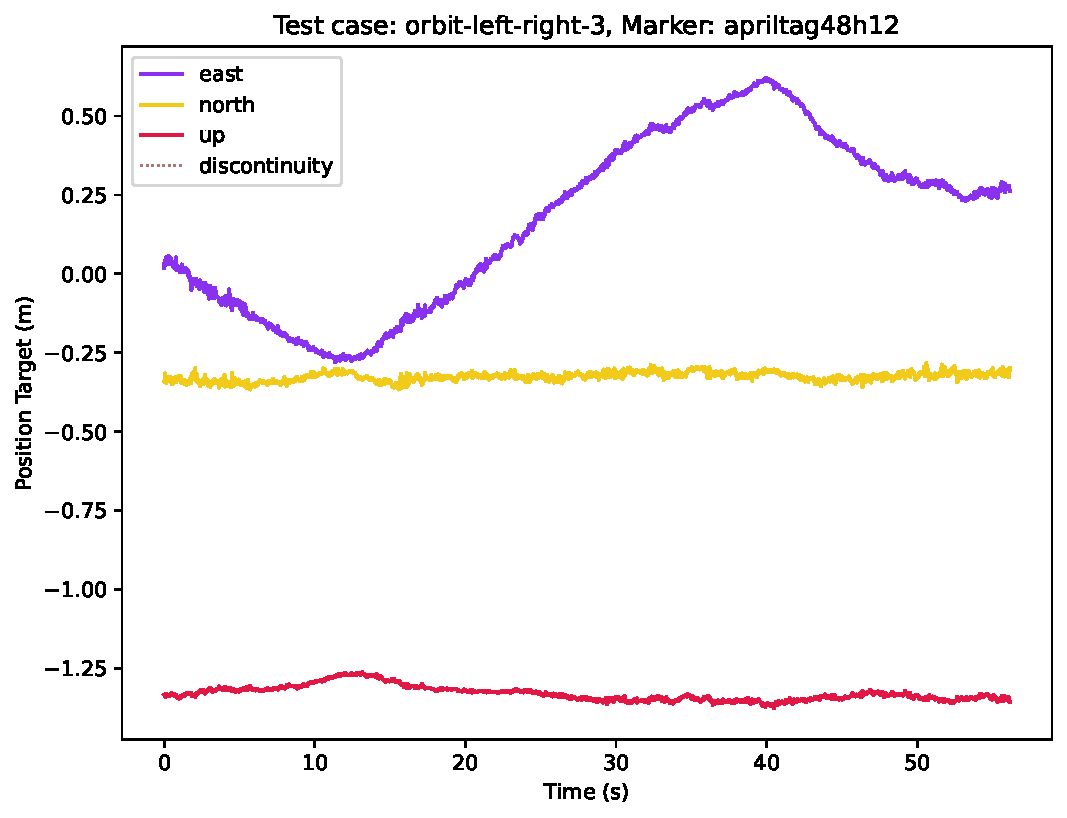
\includegraphics[width=\linewidth]{images/orbit-left-right-3_apriltag48h12_position-target}
%\end{column}
%\end{columns}
%\end{frame}
%\begin{frame}{Fiducial Markers}
%		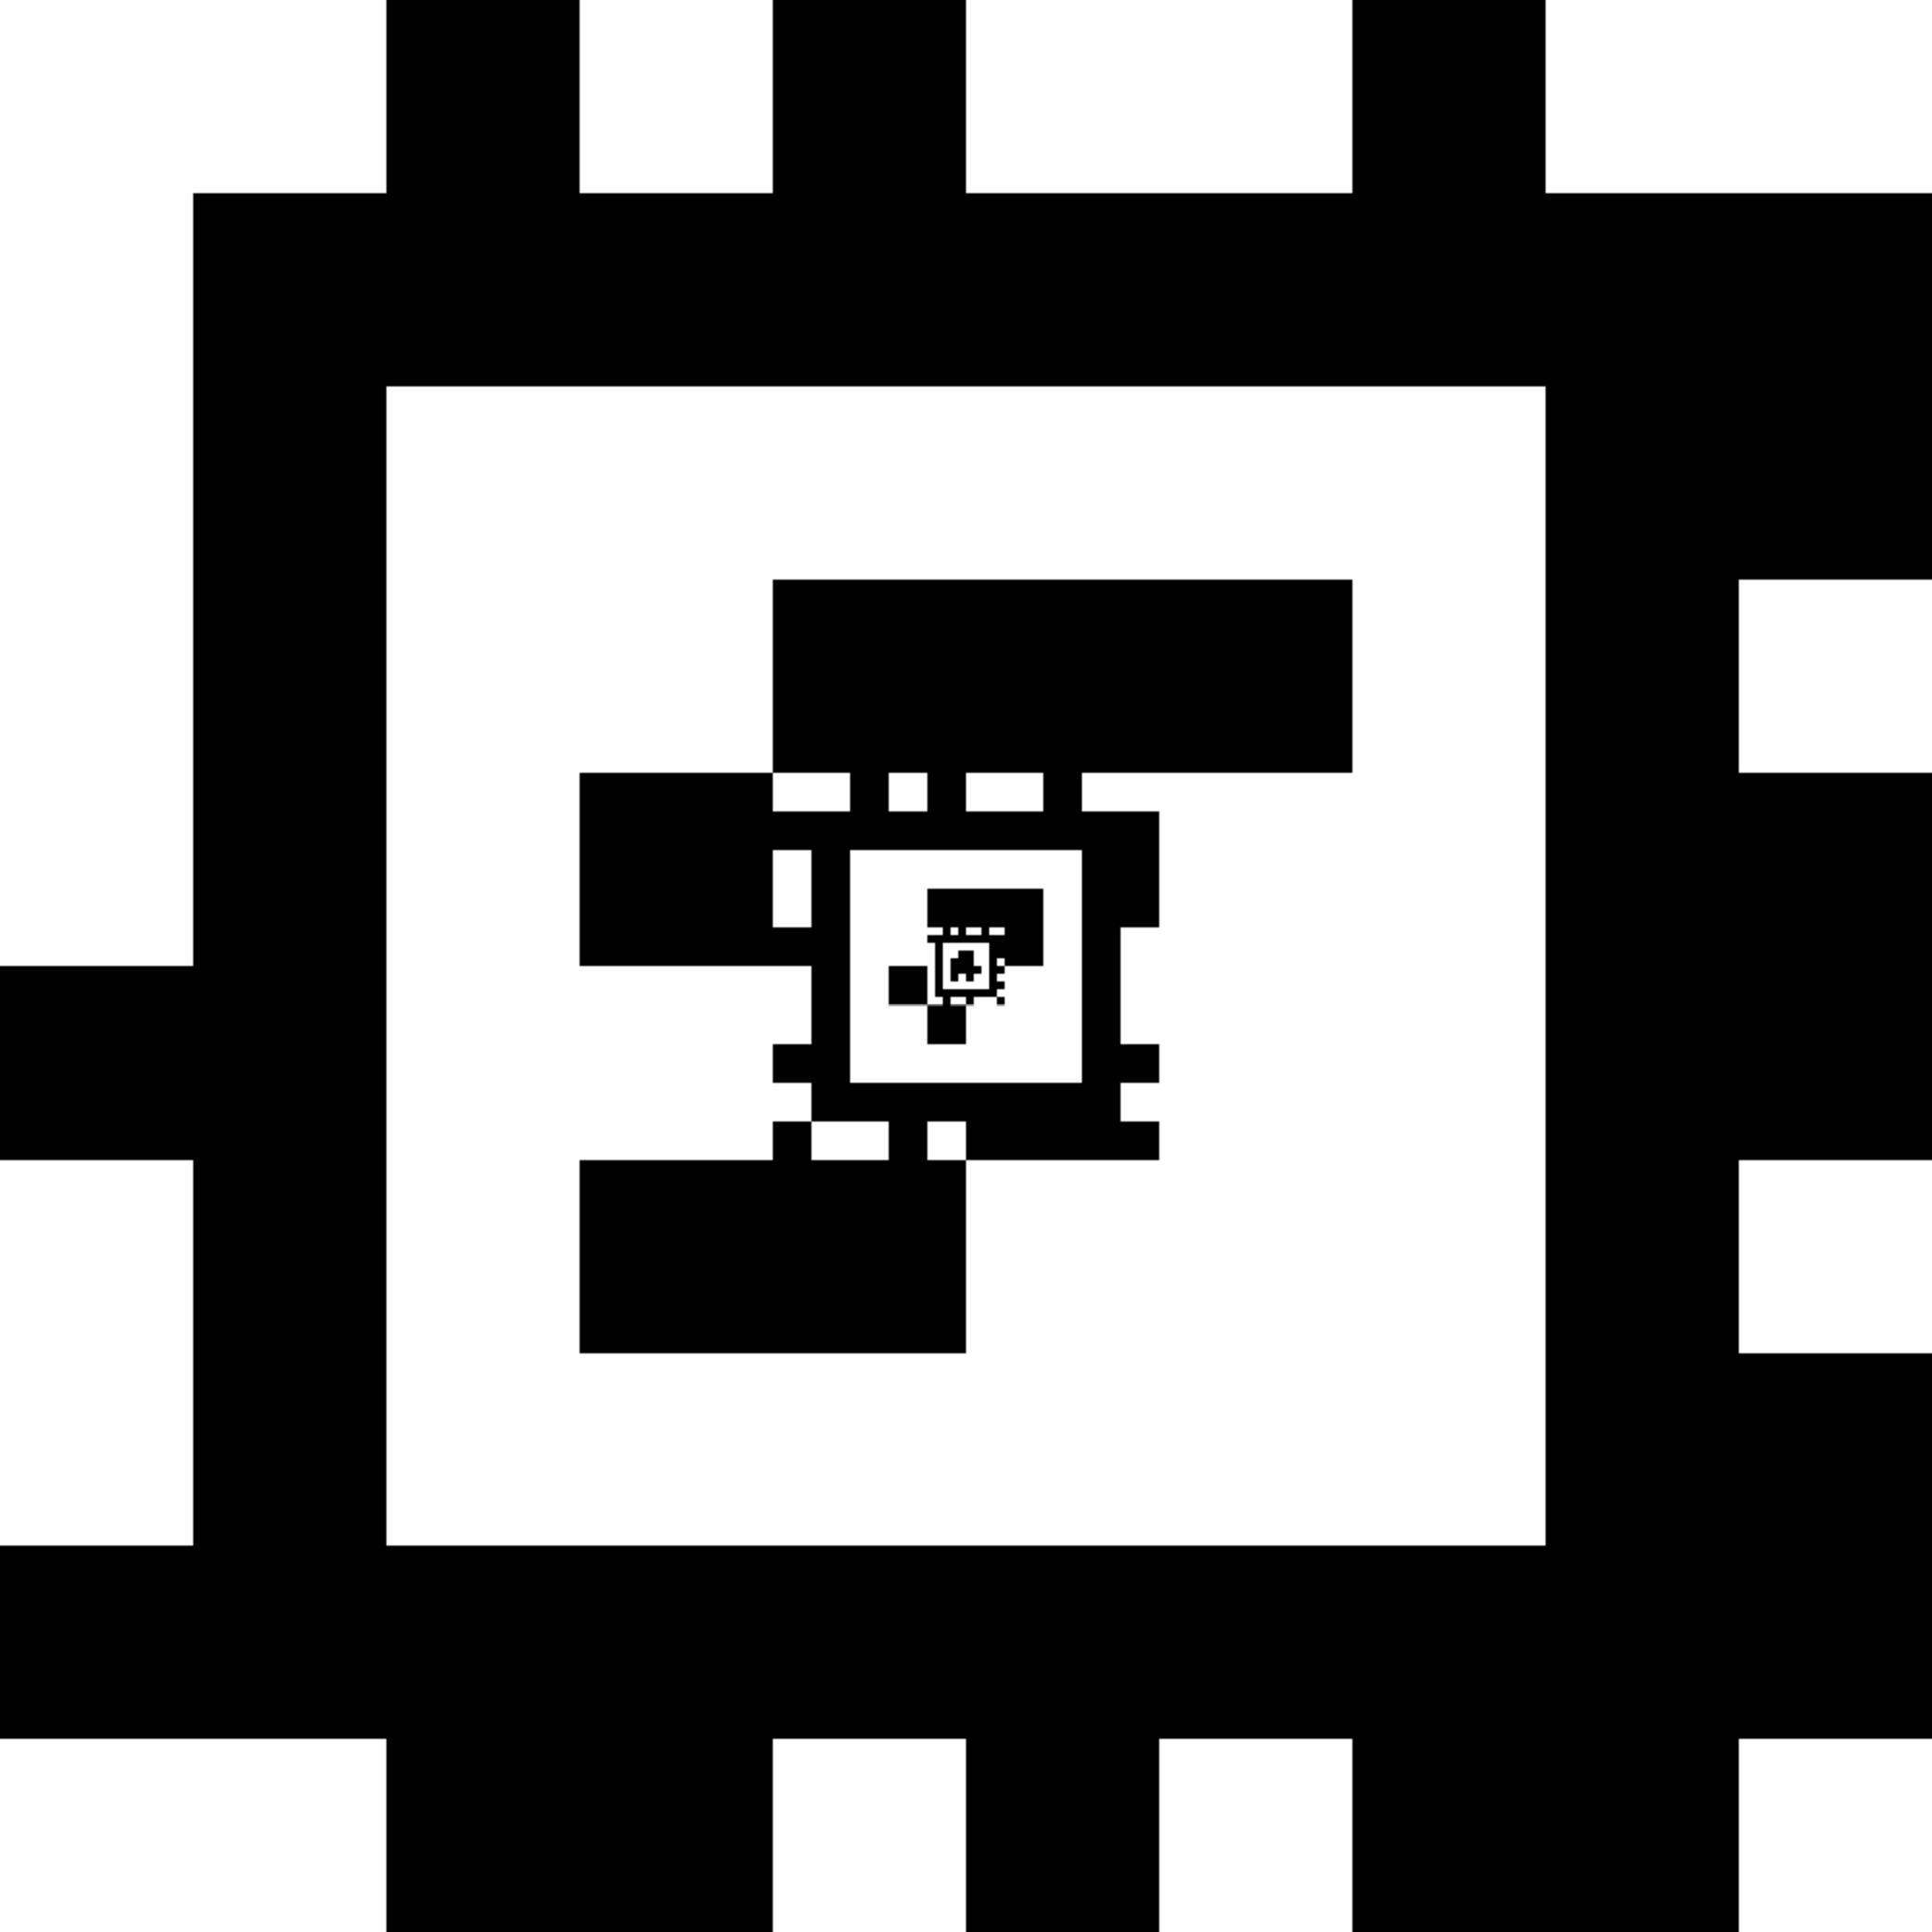
\includegraphics[width=2cm]{./images/tagCustom48h12_00002_00001_00000}
%		\includegraphics[width=2cm]{./images/tagCustom24h10_00002_00001_00000}
%		
\includegraphics[width=2cm]{./images/whycode_20_8}
%		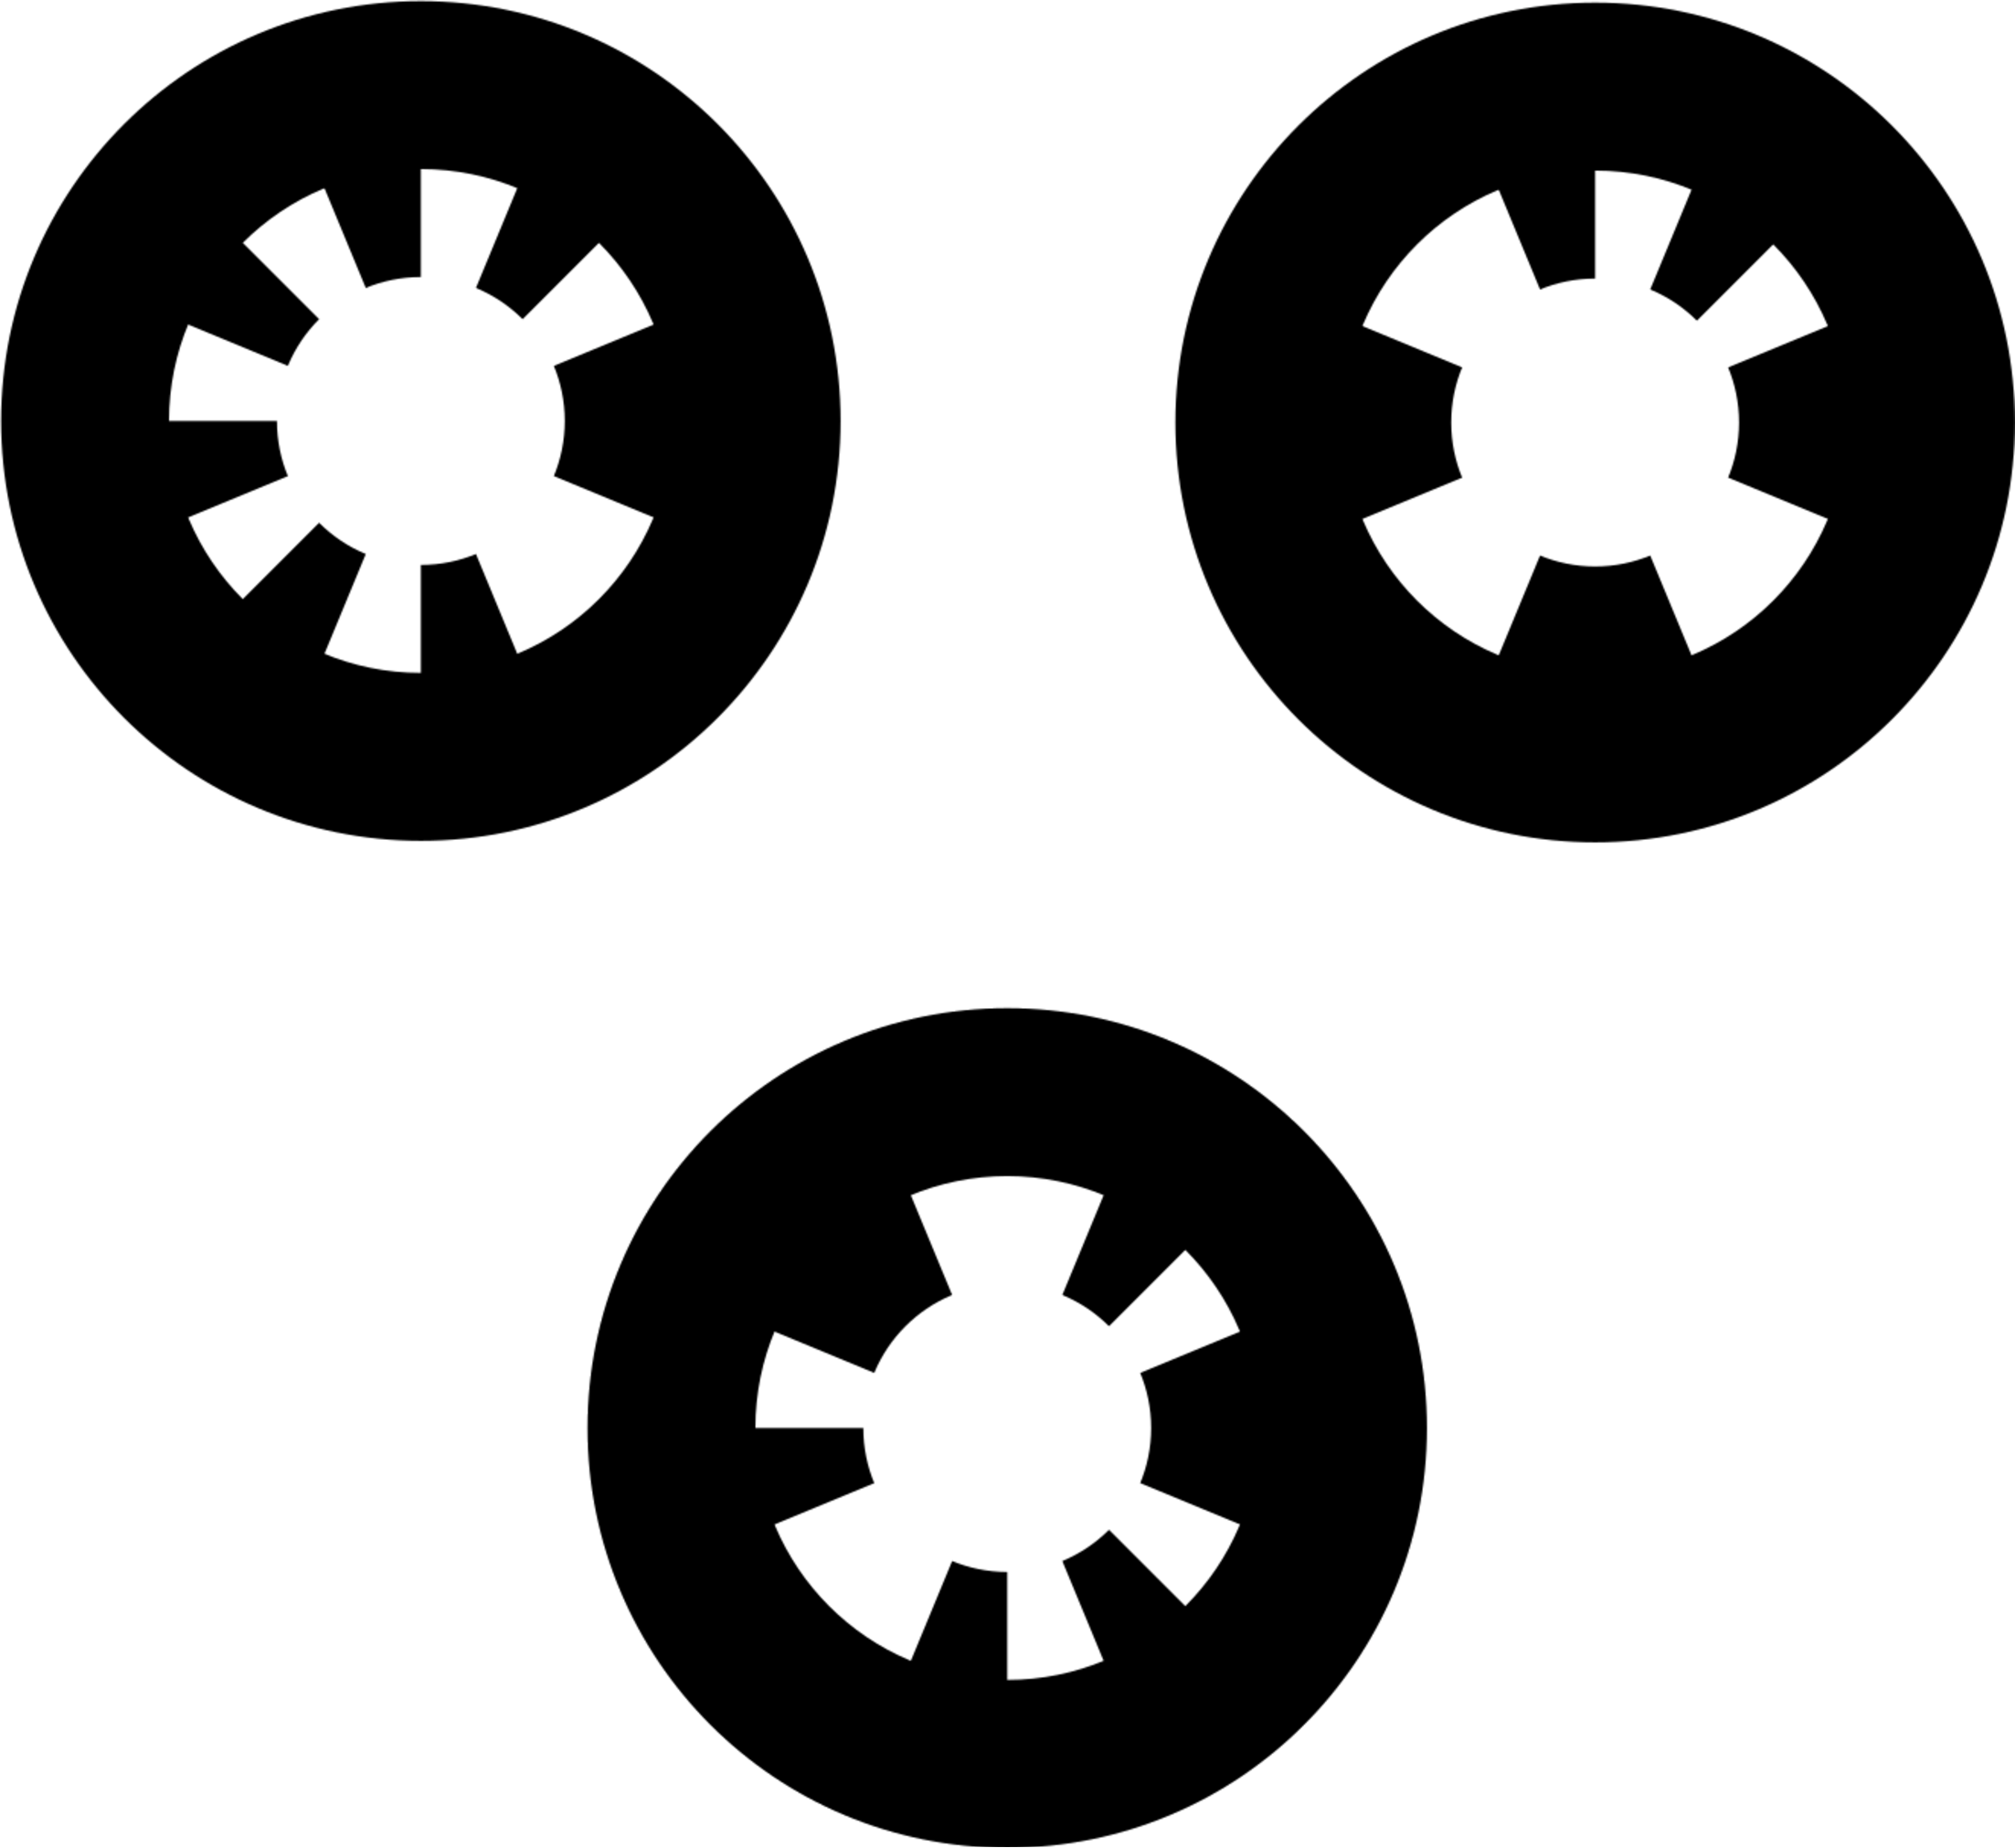
\includegraphics[width=2cm]{./images/whycode_multi}\\
%		April Tag 48h12~\footcite{apriltag3_paper}
%		April Tag 24h10%~\footcite{fiducial_precursor_evaluation}
%		WhyCode (Orig)~\footcite{whycode_paper}
%		WhyCode Multi%~\footcite{fiducial_precursor_evaluation}
%	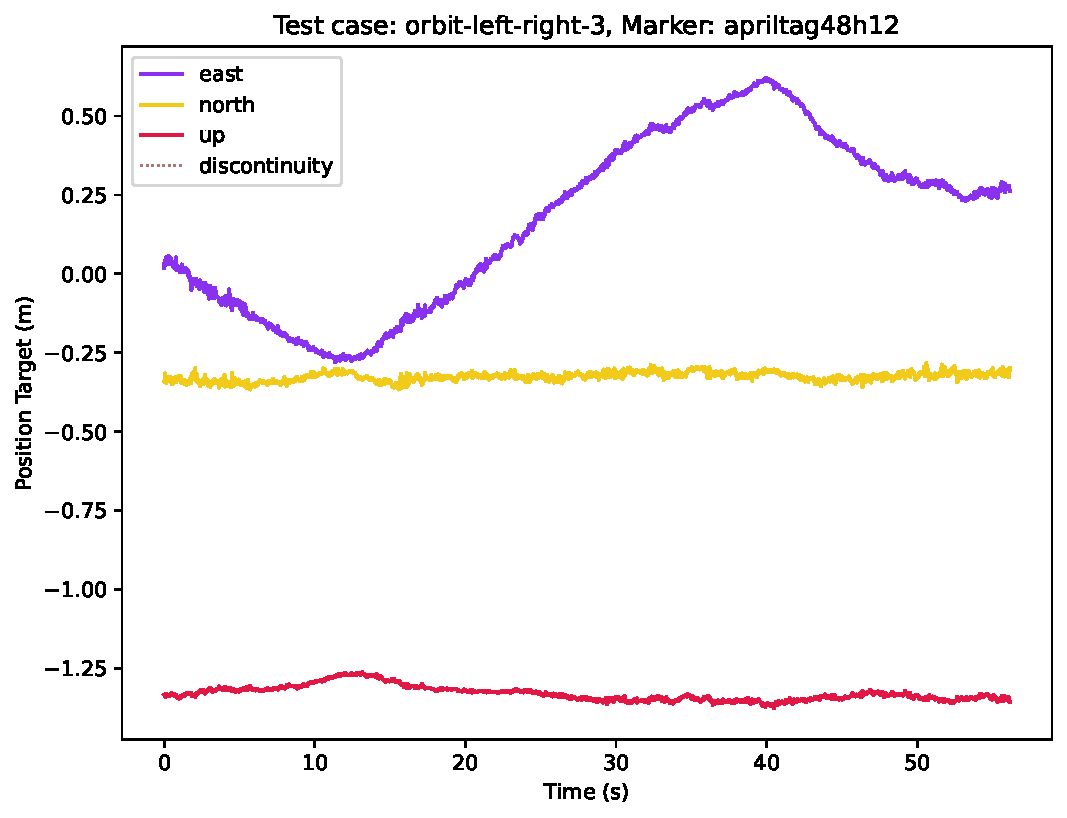
\includegraphics[width=0.3\linewidth]{images/orbit-left-right-3_apriltag48h12_position-target}
%\end{frame}

\begin{frame}{Discontinuities}
	\centering
	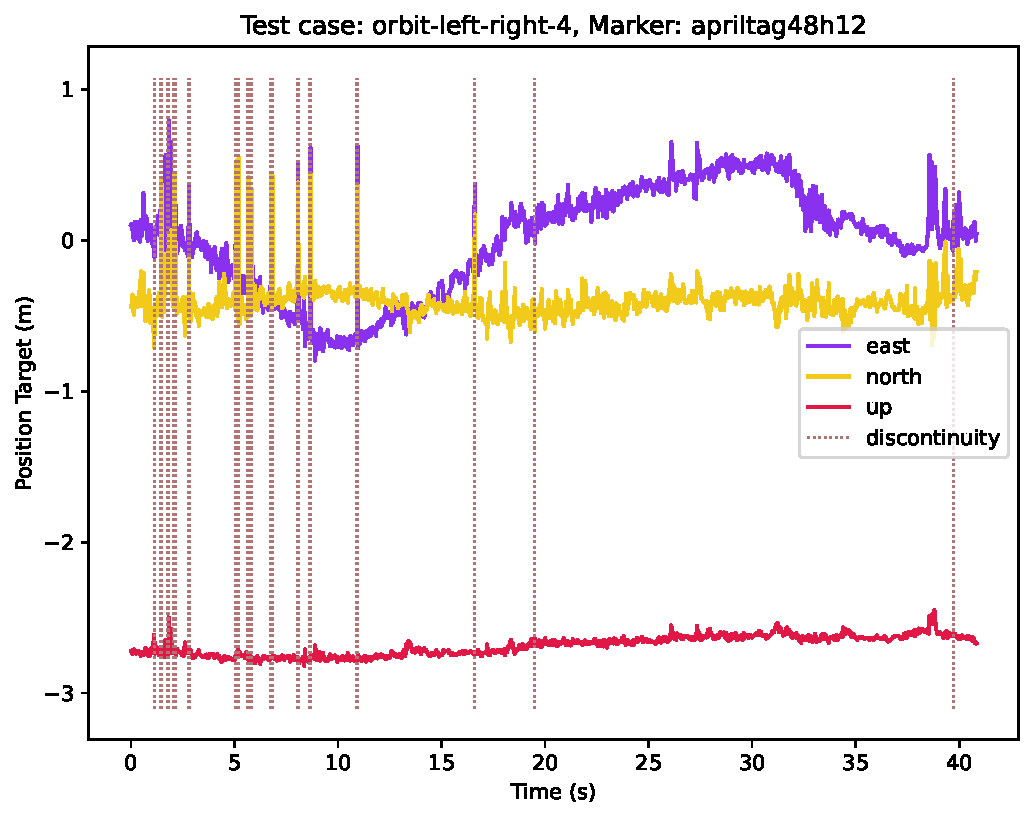
\includegraphics[width=0.75\linewidth]{images/orbit-left-right-4_apriltag48h12_position-target}
\end{frame}

\begin{frame}{Evaluation Results}
    \centering
    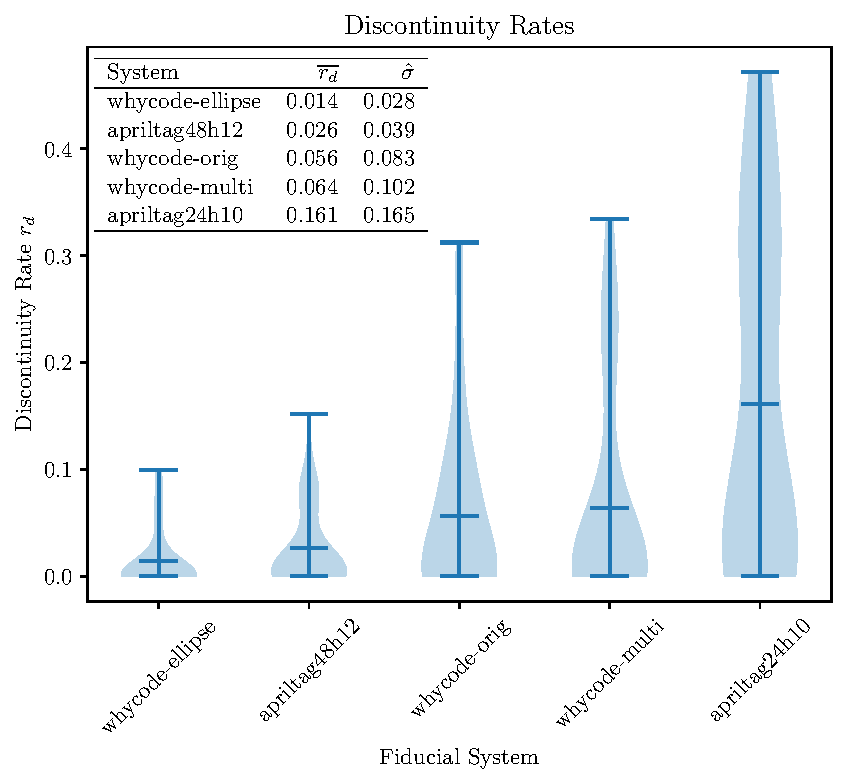
\includegraphics[width=0.49\linewidth]{./images/violin_plot_five_member}
    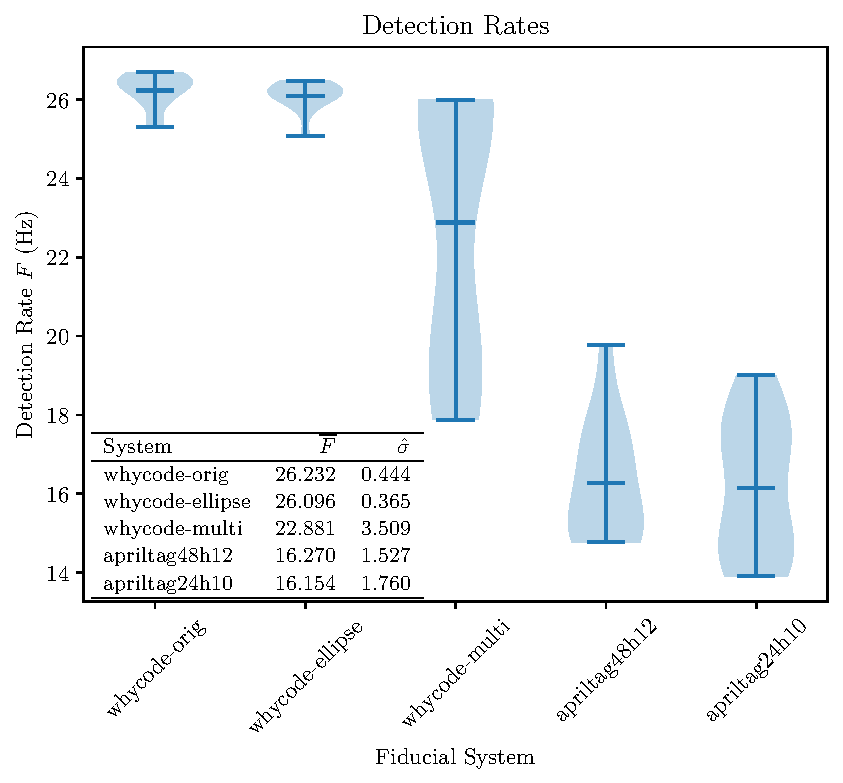
\includegraphics[width=0.49\linewidth]{./images/violin_plot_speed_five_member}
\end{frame}

\begin{frame}{Landing Pads with Fiducial Markers}
\begin{columns}
	\begin{column}{0.5\textwidth}
		\begin{figure}
		\centering
		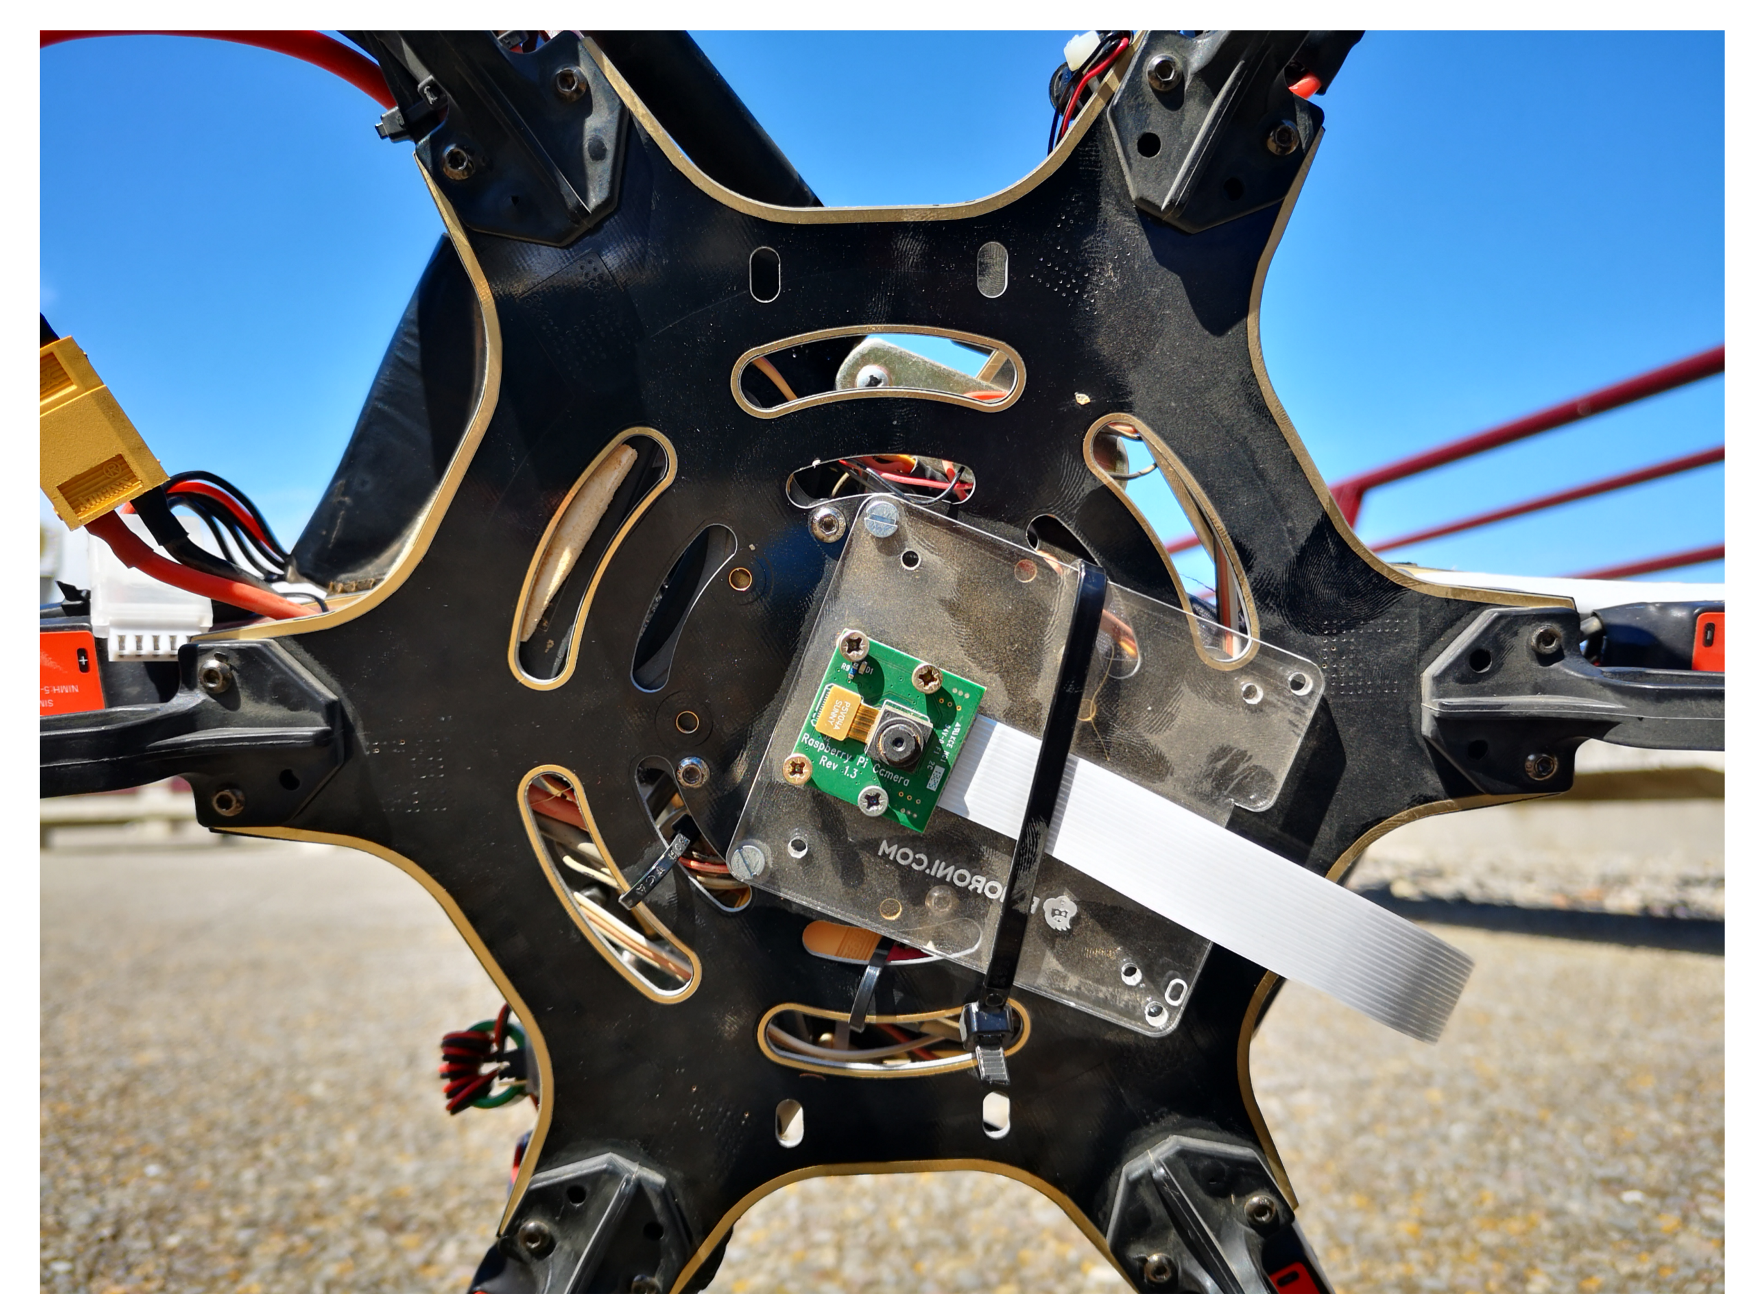
\includegraphics[width=\textwidth]{./images/wubben_drone}
		\caption{Classic, downward-facing, fixed camera.~\cite{accurate_landing_UAV_ground_pattern}}
		\label{figure:downward_facing_fixed_camera}
		\end{figure}
	\end{column}
	\begin{column}{0.5\textwidth}
	\begin{itemize}
		\item Fixed, downward-facing camera paradigm
		\item Loses sight of the landing pad in adverse conditions (e.g. wind)
	\end{itemize}
	\end{column}
\end{columns}
\end{frame}

\begin{frame}{Proof of Concept Landing with Actuated Camera}
	\centering
	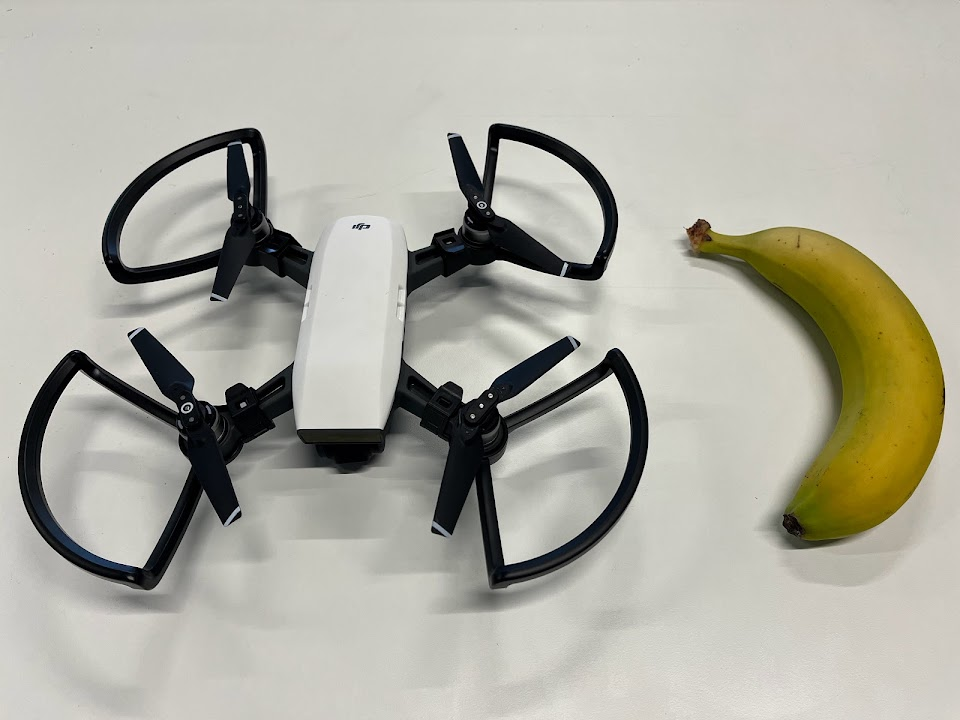
\includegraphics[height=0.55\textheight]{./images/dji_spark}
	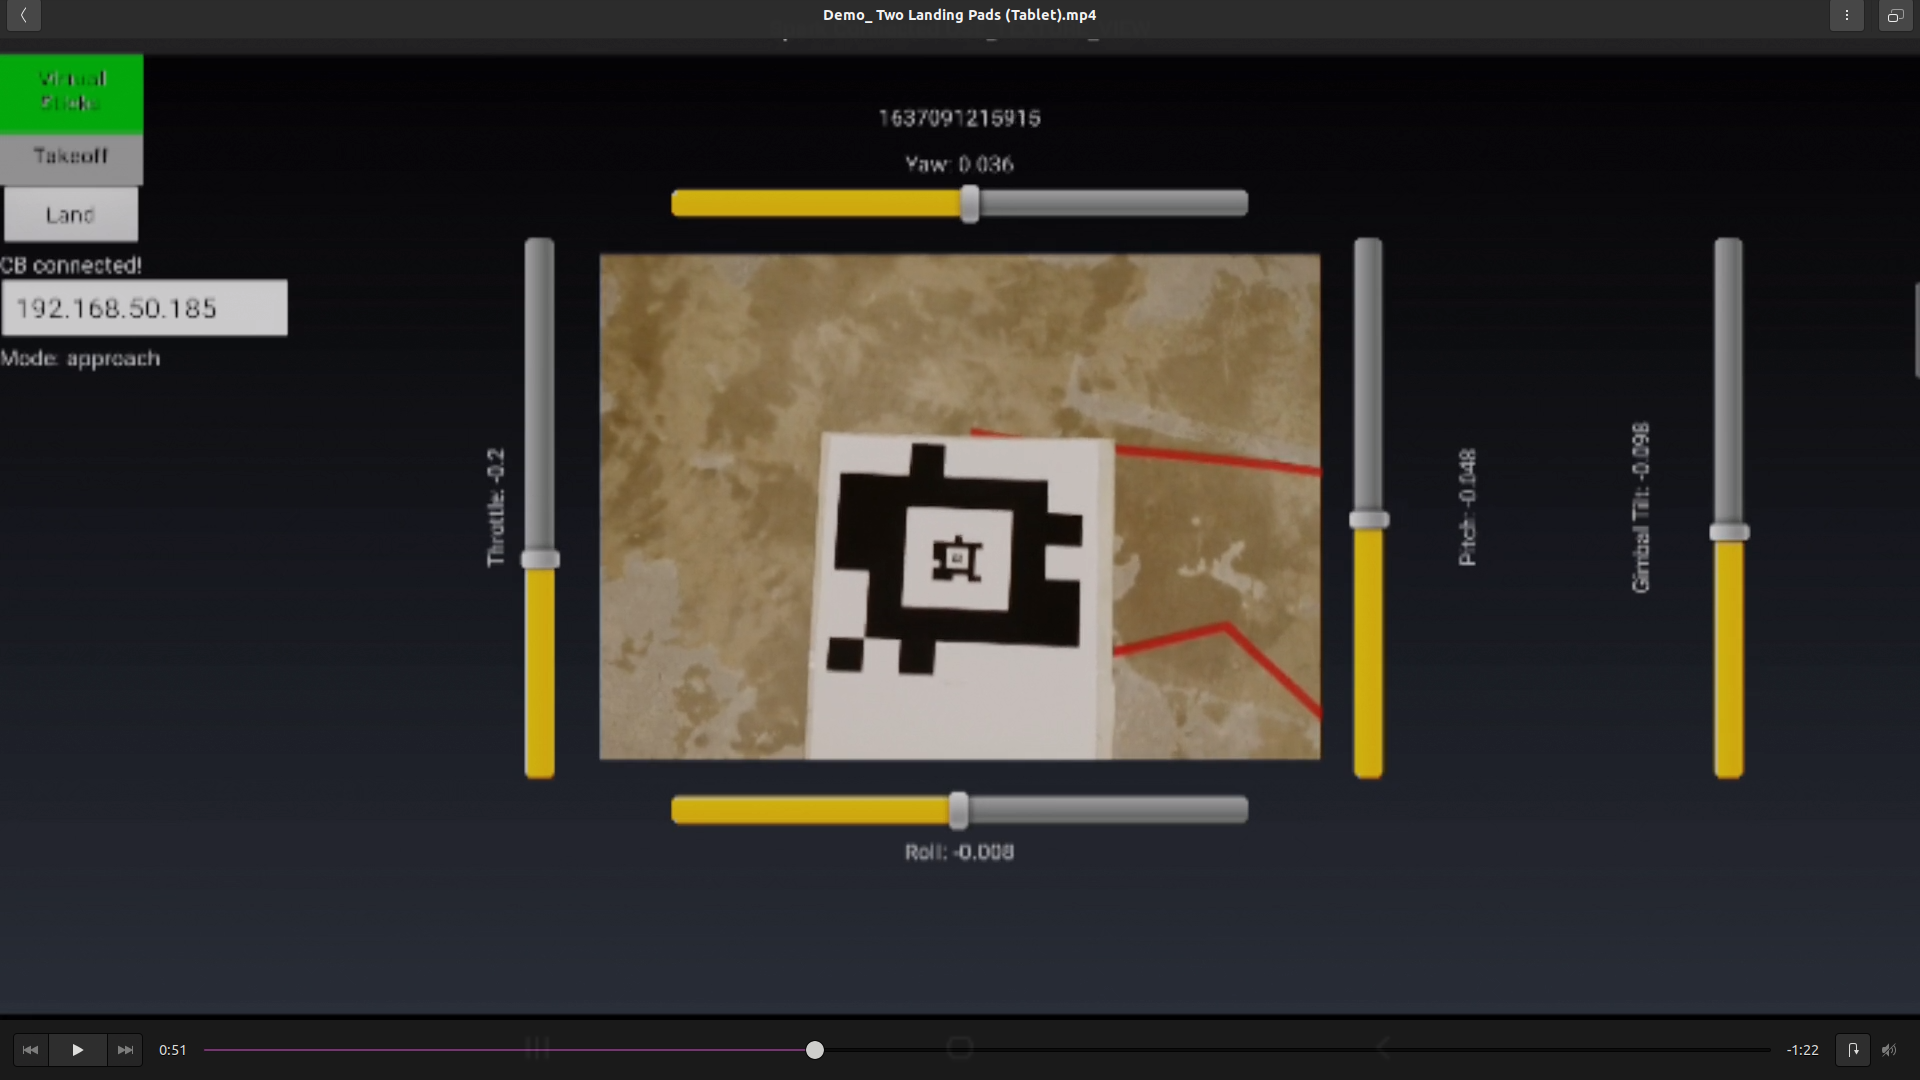
\includegraphics[height=0.55\textheight]{./images/tablet_screenshot}
	\href{run:./autonomous_landing_demonstration_short.mp4}{Demonstration Video}
\end{frame}

%\begin{frame}{Tracking Performance Example}
%	\centering
%	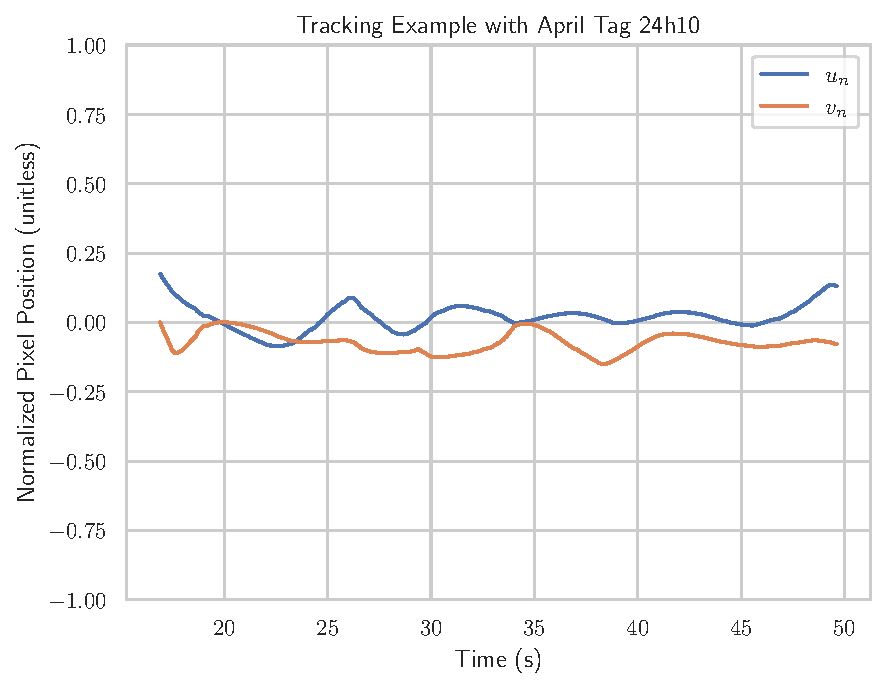
\includegraphics[height=\textheight]{./images/tracking_example}
%\end{frame}
%
%\begin{frame}{Trajectory and Control Signals}
%    \centering
%    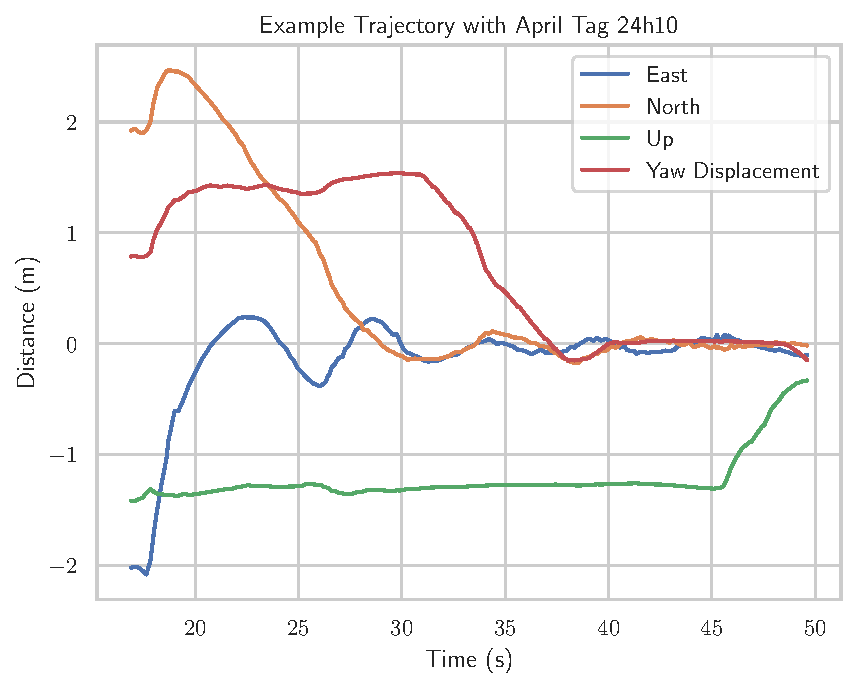
\includegraphics[width=0.49\textwidth]{./images/landing_trajectory}
%    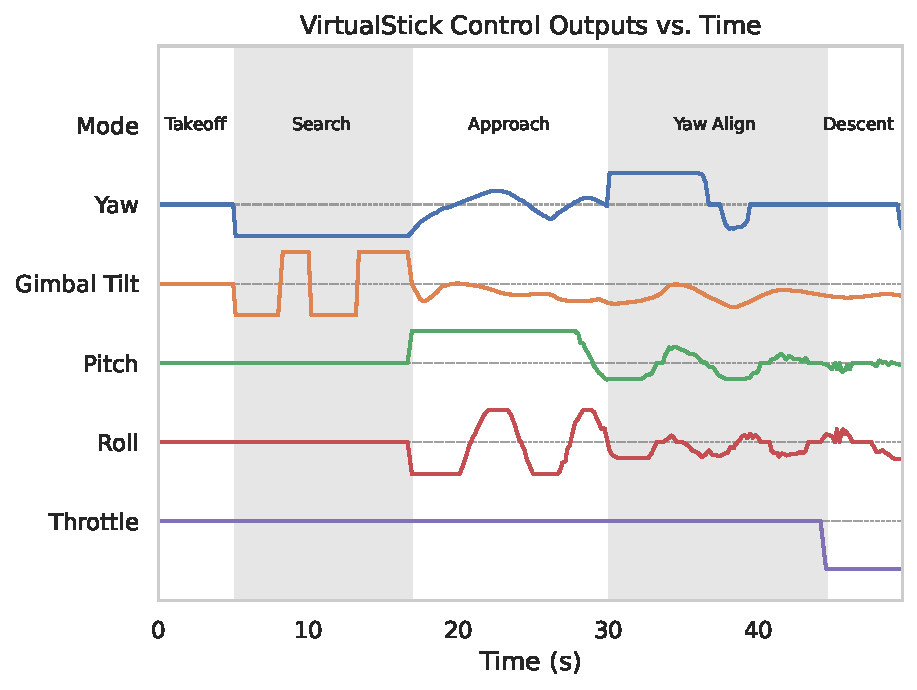
\includegraphics[width=0.49\textwidth]{./images/control_example}
%\end{frame}
%
%\begin{frame}{Trajectory and Control Signals (With Discontinuities)}
%    \centering
%    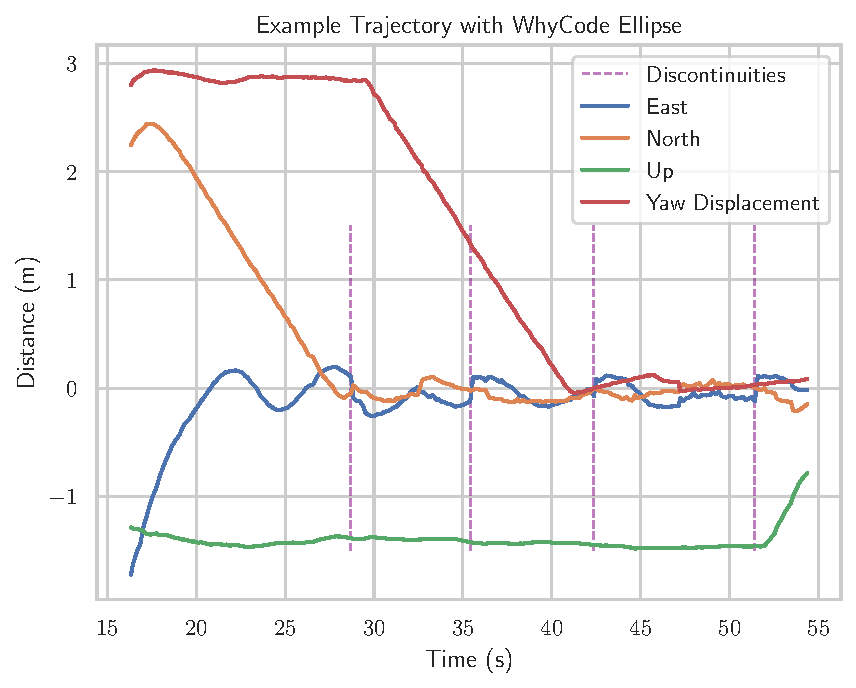
\includegraphics[width=0.49\textwidth]{./images/landing_trajectory_with_discontinuities}
%    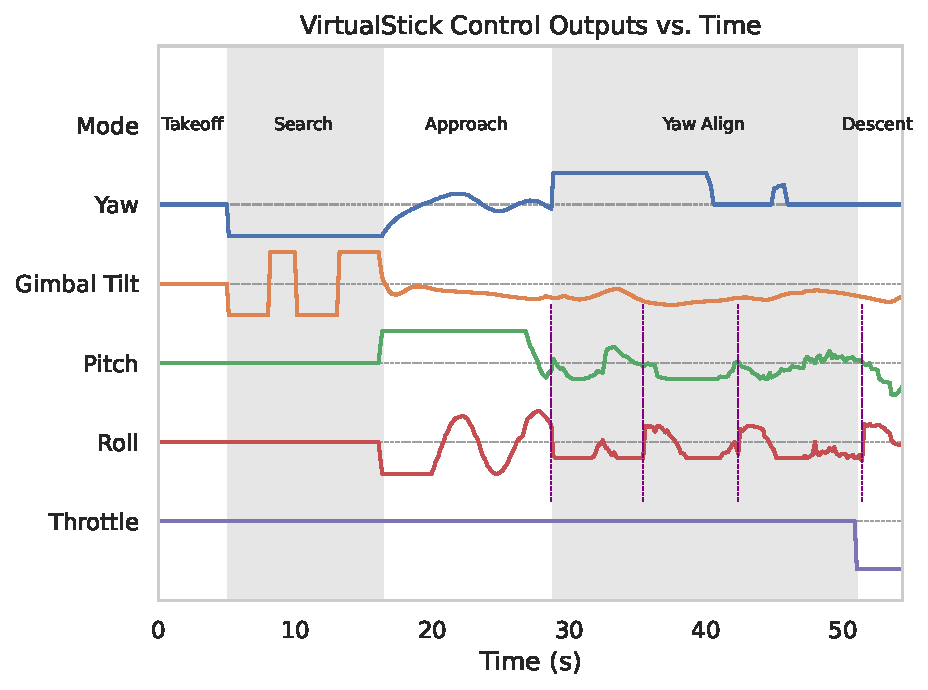
\includegraphics[width=0.49\textwidth]{./images/control_example_with_discontinuities}
%\end{frame}
%
%\begin{frame}{Overall Performance}
%	\centering
%	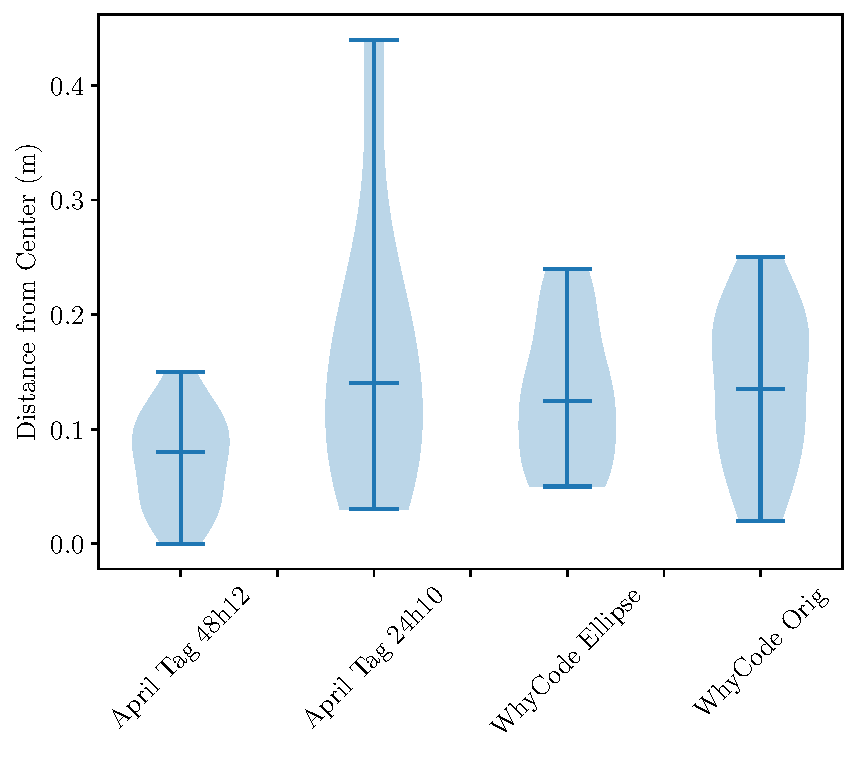
\includegraphics[height=\textheight]{./images/violin_plot_landing_radii}
%\end{frame}
\begin{frame}{Future Work: Fiducial Tests}
\begin{columns}
	\begin{column}{0.5\textwidth}
	\begin{itemize}
		\item Re-conduct fiducial landing tests with actuated camera
		\item Raw pose data (same as before)
		\item Filtered pose data (KF, etc)
		\item Hybrid data
		\begin{itemize}
			\item Position from marker
			\item Orientation from camera gimbal
		\end{itemize}
	\end{itemize}
	\end{column}
	\begin{column}{0.5\textwidth}
		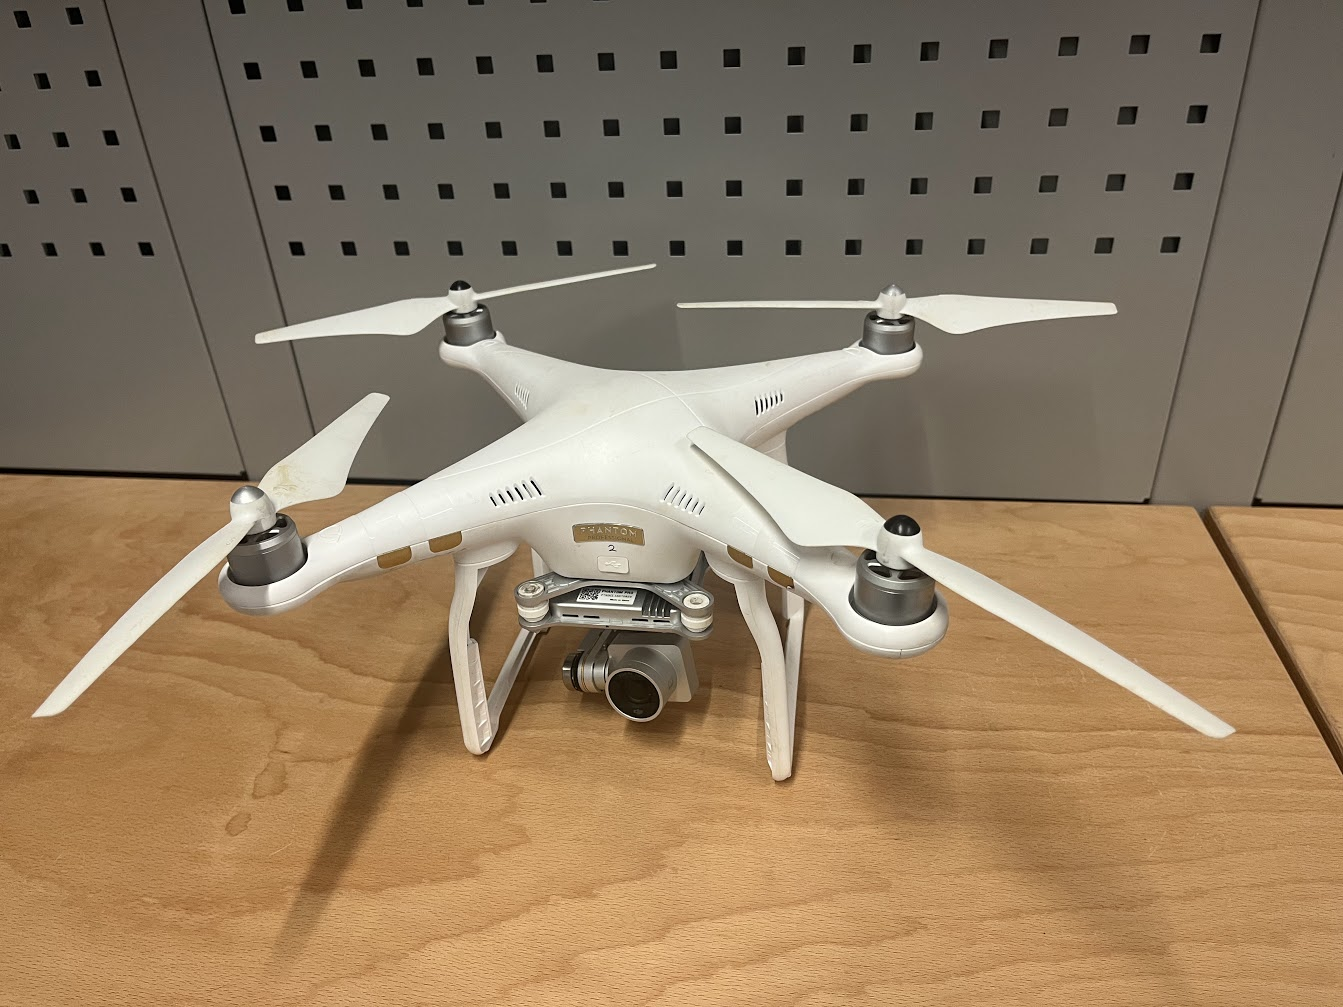
\includegraphics[width=\textwidth]{./images/phantom_3}
	\end{column}
\end{columns}
\end{frame}

\section{Unstructured Case: Lava Flows}

\begin{frame}{RAVEN, Mars Analog Missions in Iceland}
	\centering
	\includegraphics[width=10cm]{./images/raven_rover_drone}

	{\tiny\fullcite{Bapst2021Mars}}
\end{frame}

\begin{frame}{RAVEN, Mars Analog Missions in Iceland}
	\centering
	\includegraphics[height=0.55\textheight]{./images/holuhraun_aerial}
	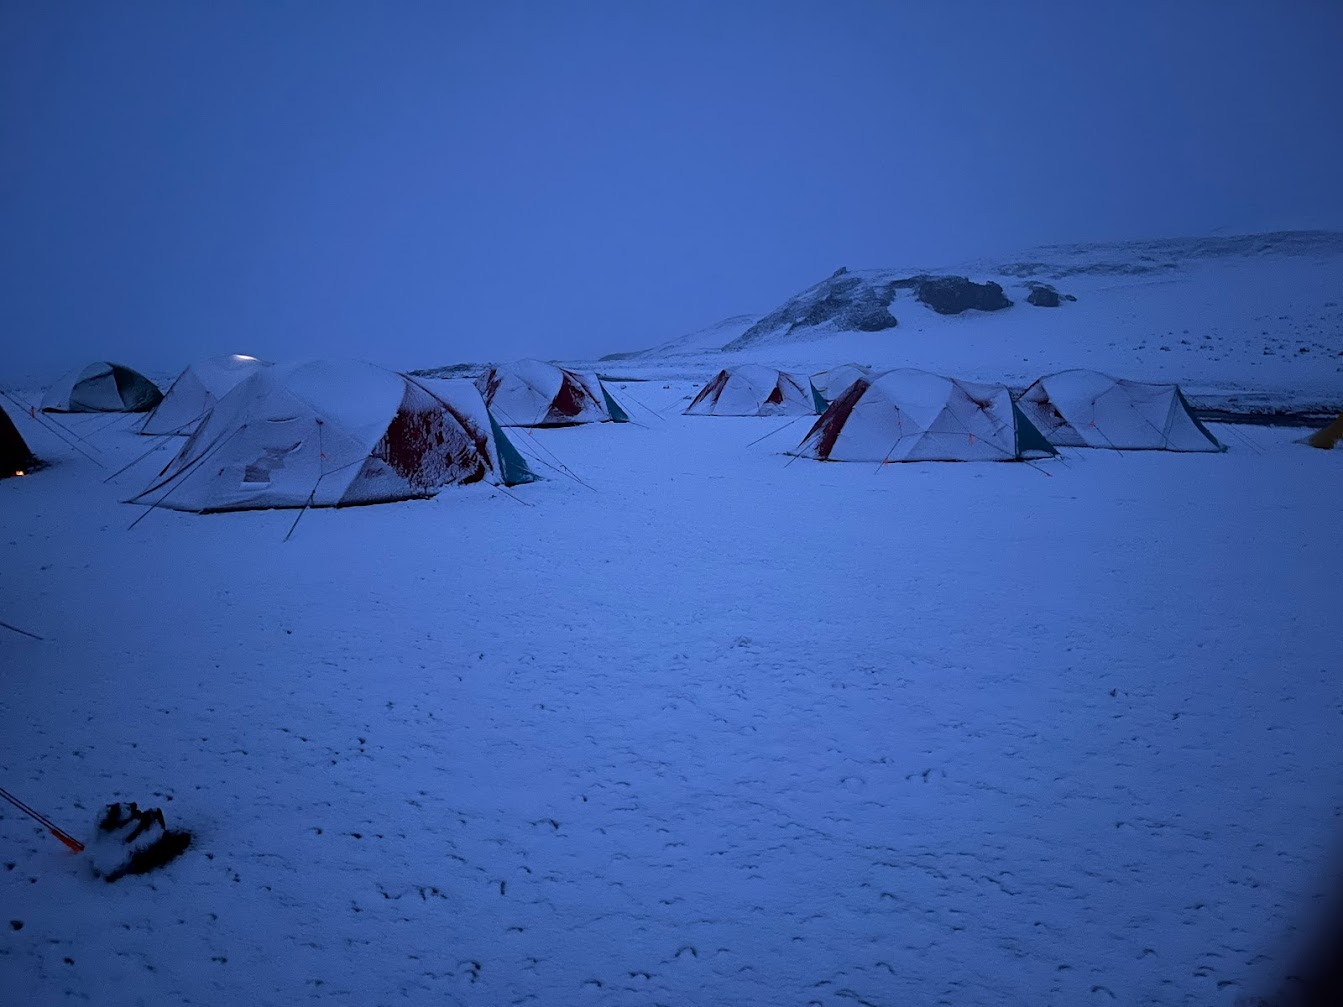
\includegraphics[height=0.55\textheight]{./images/dreki_small_tents_snow}
\end{frame}

\begin{frame}{Lava Flow Landings}
	\centering
	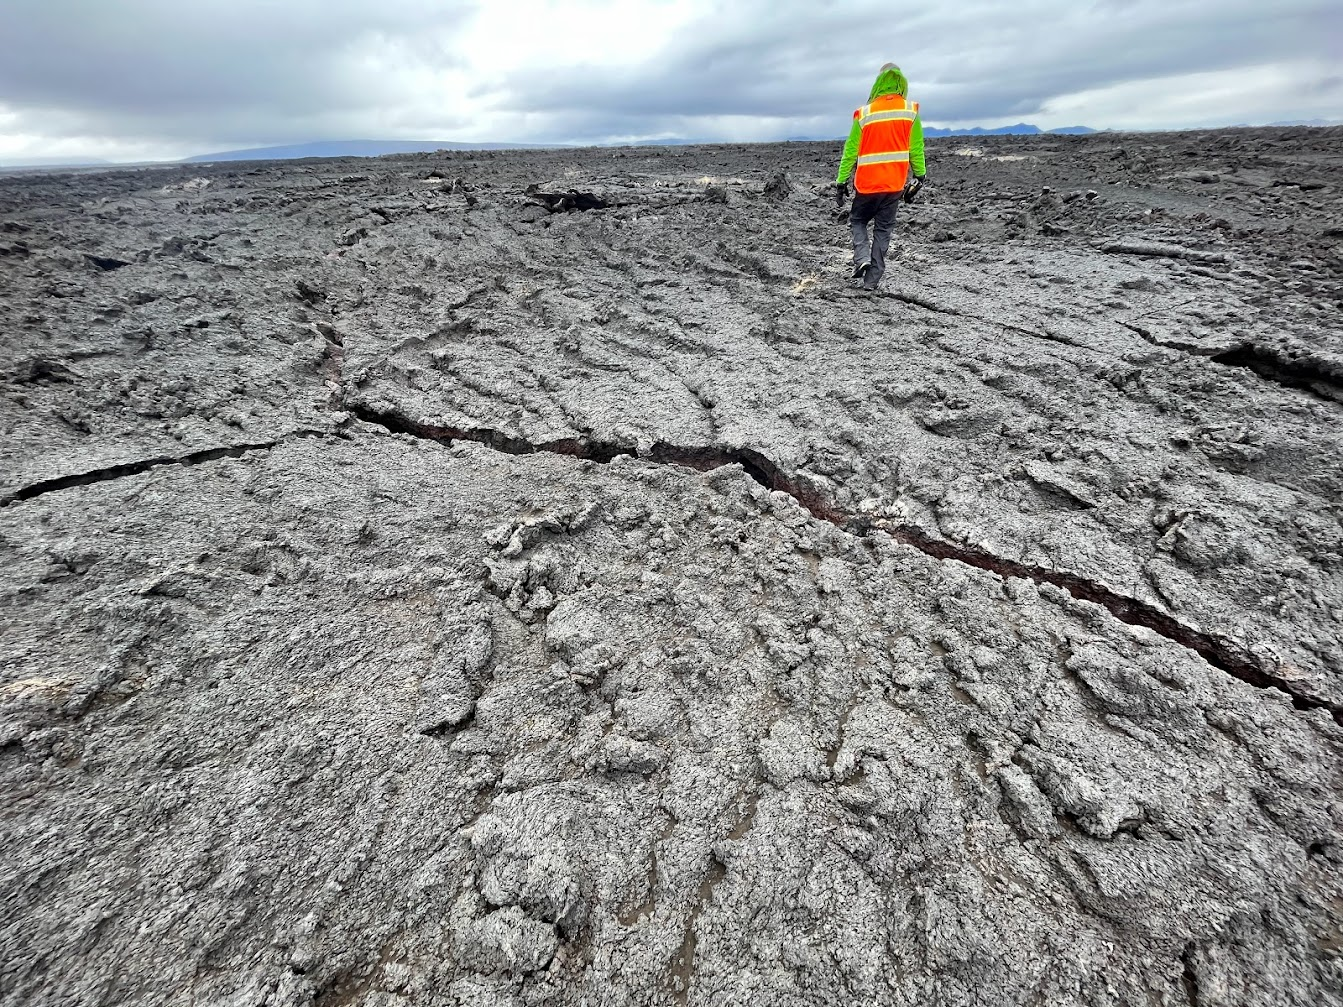
\includegraphics[width=0.49\textwidth]{./images/holuhraun_smooth}
	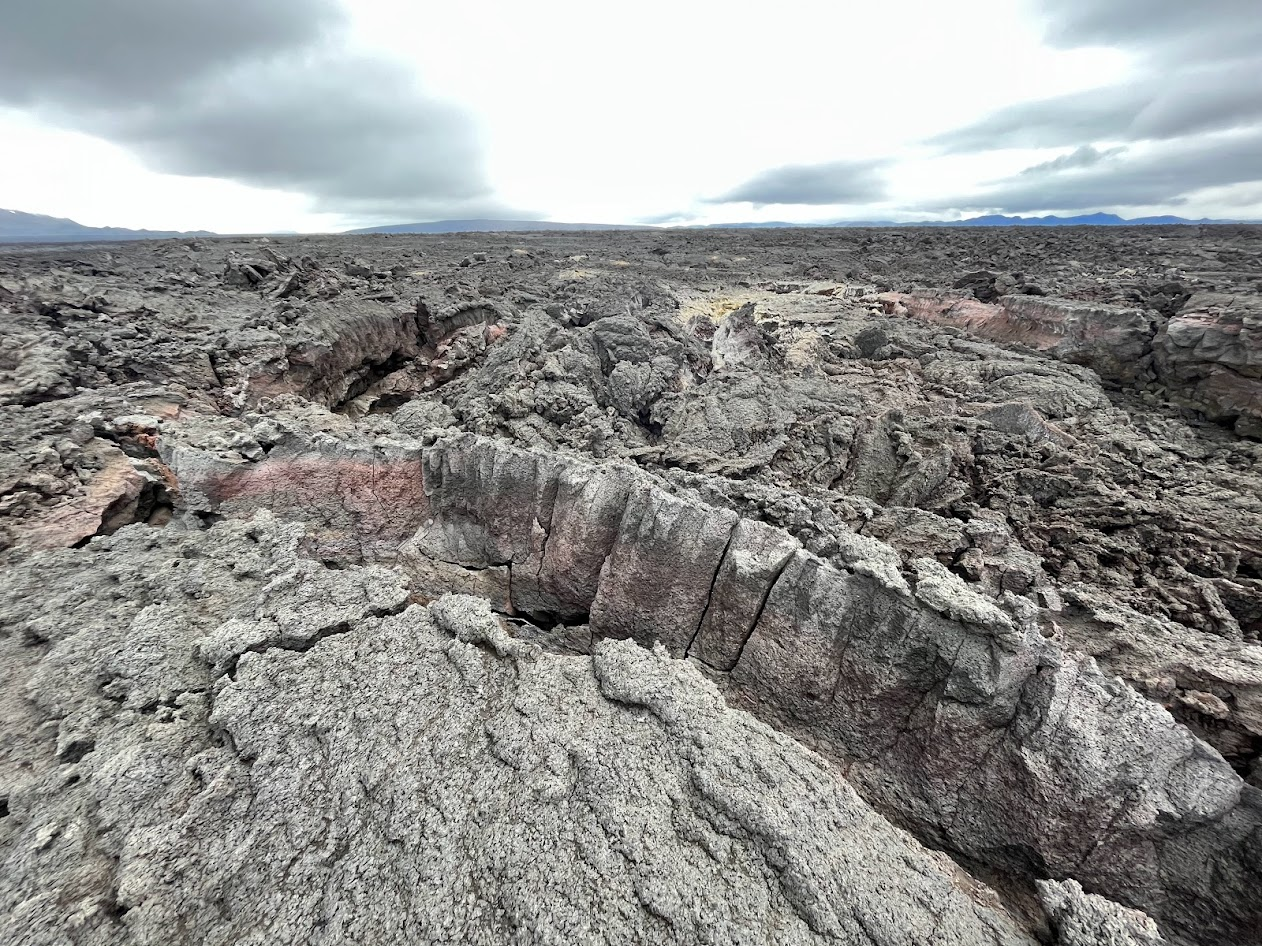
\includegraphics[width=0.49\textwidth]{./images/holuhraun_rough}

	\href{run:./lava_landing.mp4}{Manual Lava Landing Video}
\end{frame}

%\section{Moving Forward}

\begin{frame}{Reykjavík University = No-Fly Zone}
	\centering
	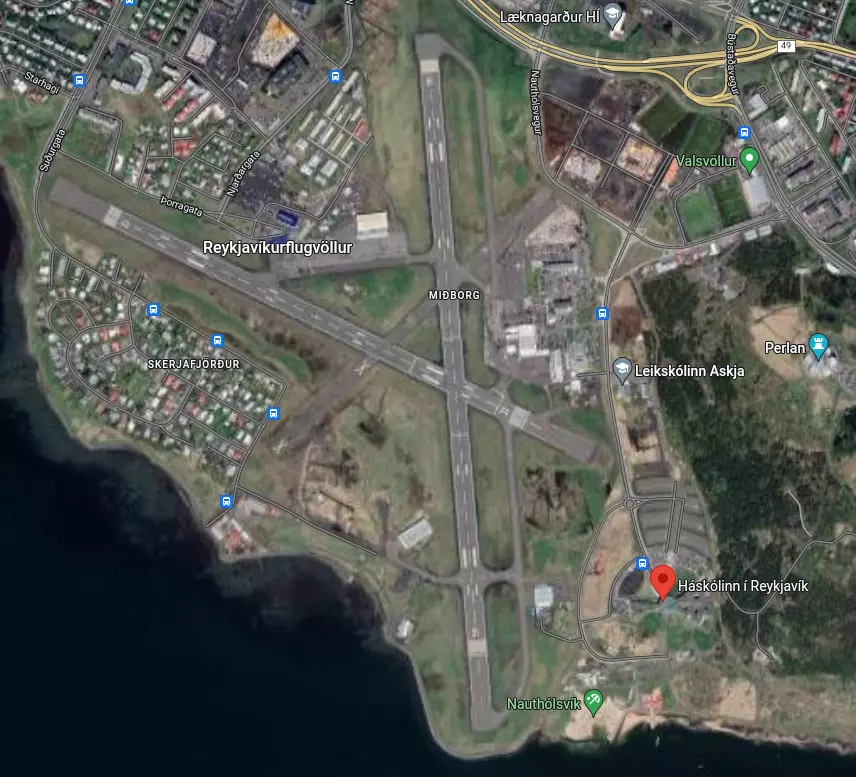
\includegraphics[height=0.6\textheight]{./images/reykjavik_university_no_fly_zone}
	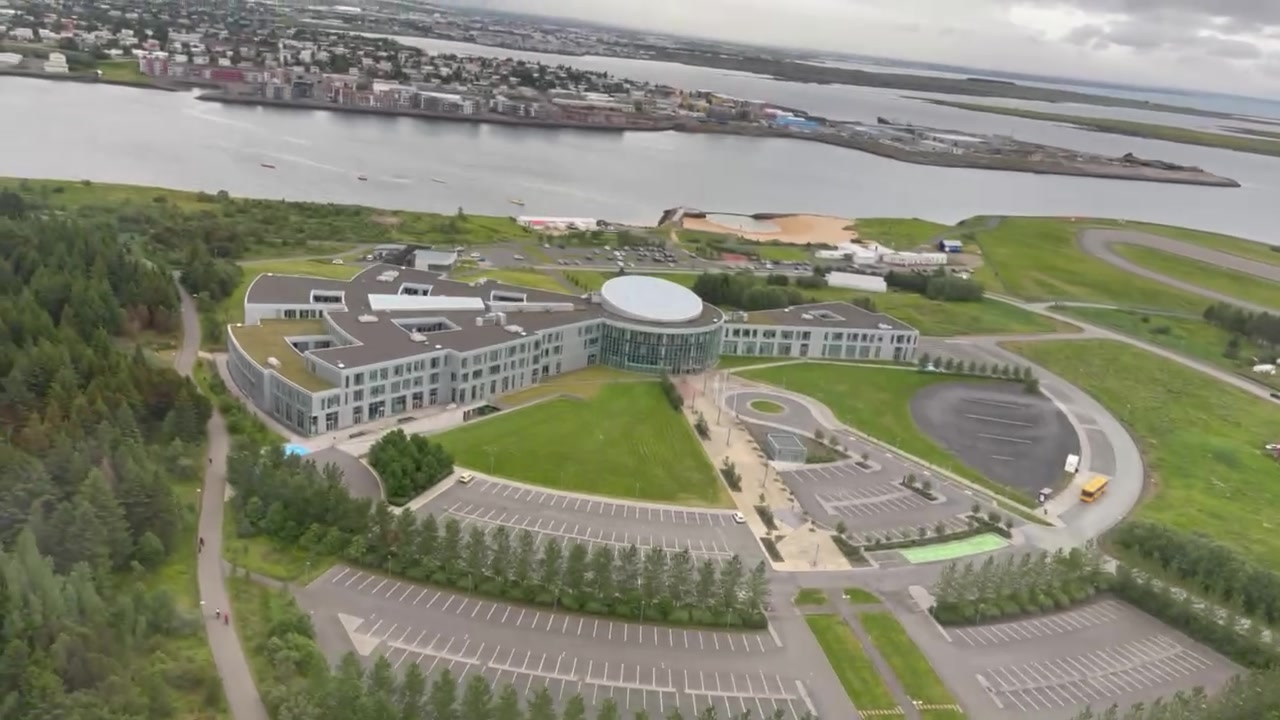
\includegraphics[height=0.6\textheight]{./images/ru_aerial.jpg}
\end{frame}

\begin{frame}{Lava Flow Landing Data Collection Area: Stóra-Bolluhraun}
	\centering
	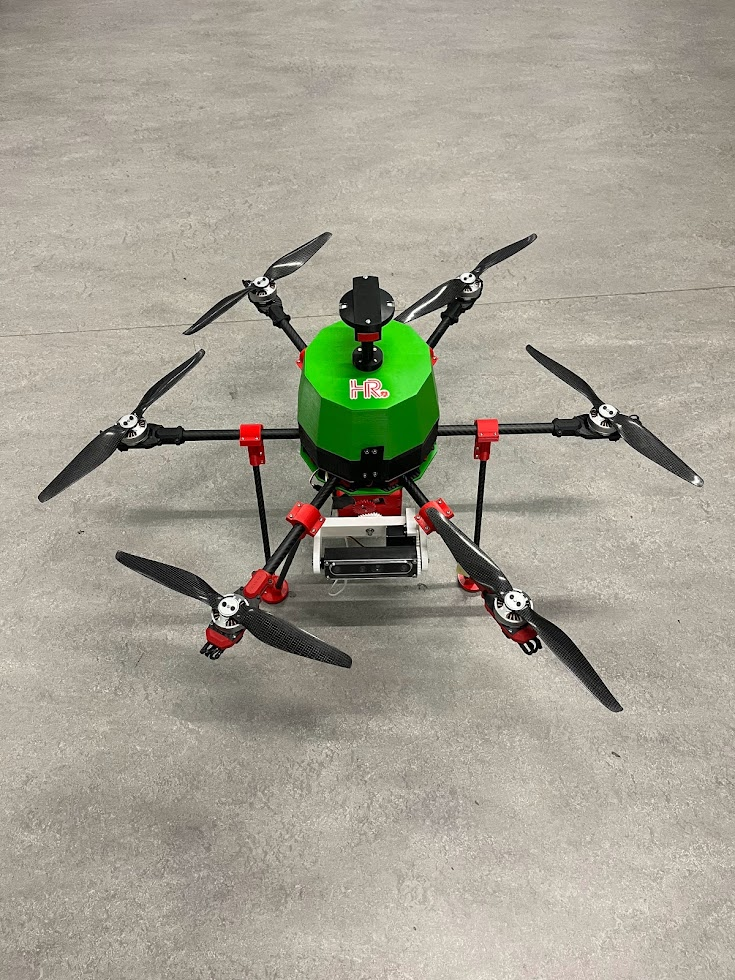
\includegraphics[height=0.8\textheight]{./images/depth_drone_sitting}
	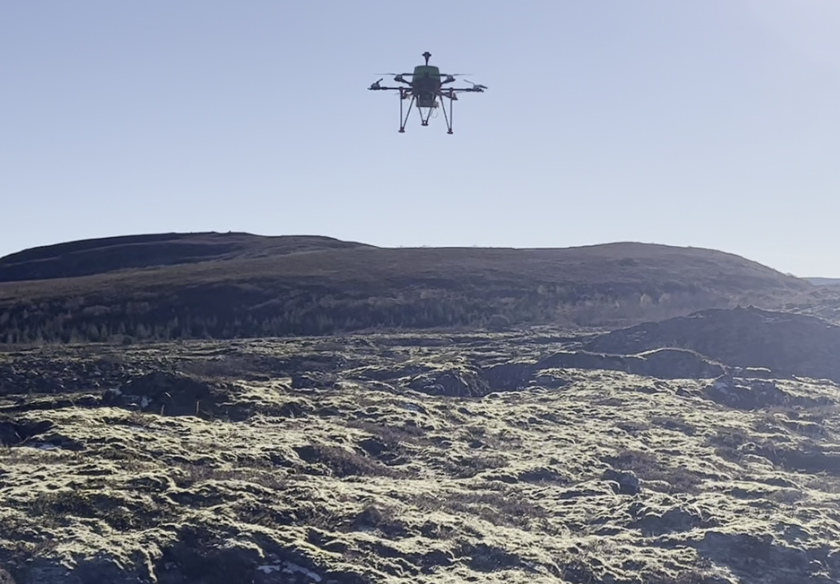
\includegraphics[height=0.8\textheight]{./images/depth_drone_flying}
%	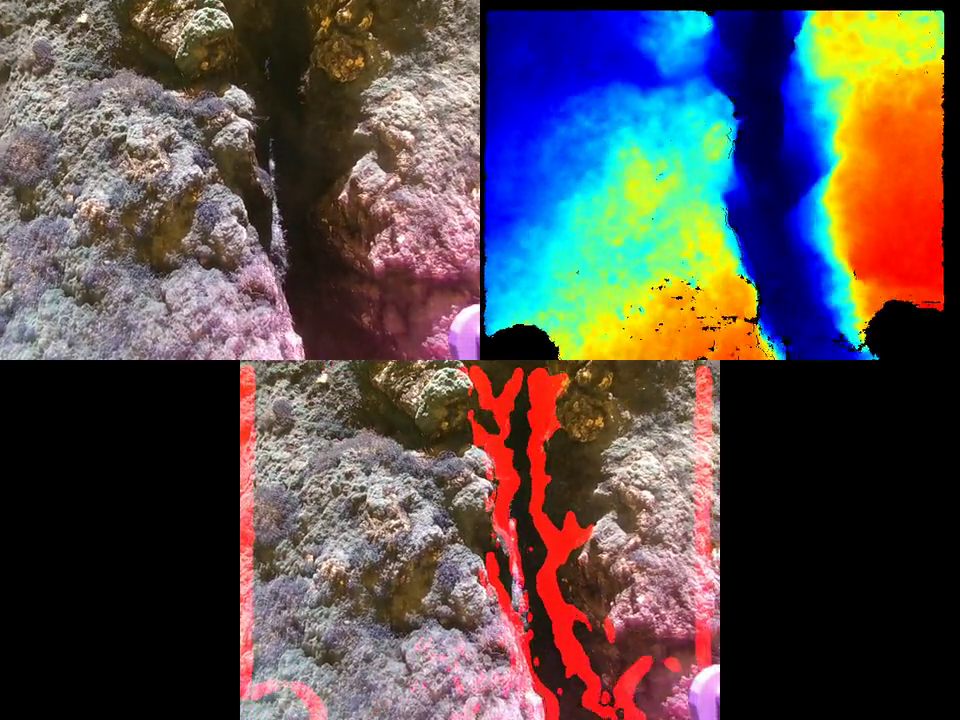
\includegraphics[height=0.6\textheight]{./images/depth_processing_screenshot}
	\\
	\href{run:./scratch_idea_for_processing_depth_data.mp4}{Data Collection Video}
\end{frame}

%\begin{frame}{Example Depth Image Processing}
%	\centering
%	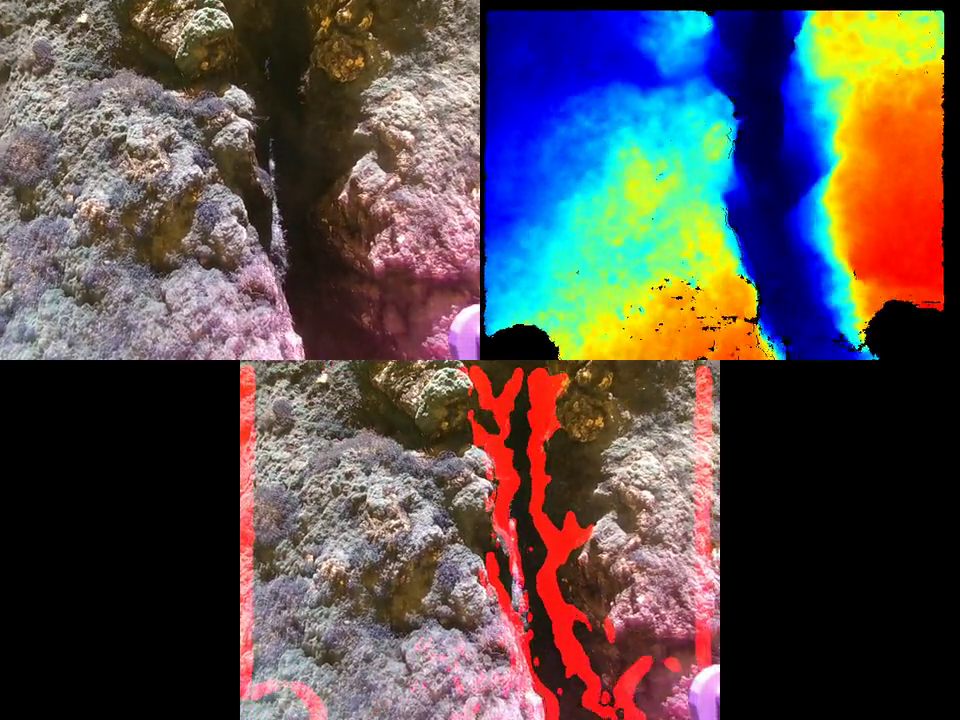
\includegraphics[height=\textheight]{./images/depth_processing_screenshot}
%\end{frame}

\begin{frame}{Moving Forward}
	\begin{itemize}
		\item Transform depth image using IMU
		\item Conventional signal processing techniques
		\item Possible: Deep learning (embedded TPU/GPU)
		\item Synthetic data generation using LIDAR point clouds: AirSim
		\item Analog$^2$ Missions
		\item New lava flows + ground penetrating RADAR
		\item Combine fiducial and lava flow methods into a single platform
	\end{itemize}
\end{frame}

\begin{frame}{Main Messages}
\begin{columns}
	\begin{column}{0.4\textwidth}
		\centering
		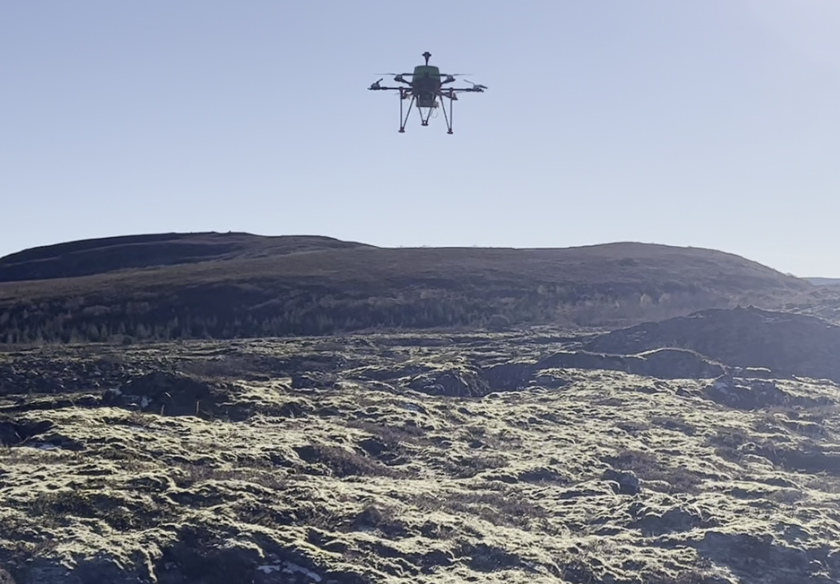
\includegraphics[width=\textwidth]{./images/depth_drone_flying}
		\vfill
		
\includegraphics[width=0.5\textwidth]{./images/qr_uzgit_github_io.png}
	\end{column}
	\begin{column}{0.6\textwidth}
	\begin{itemize}
		\item Topic: autonomous drone control -- landing
		\item Methods:
		\begin{itemize}
			\item Fiducial markers with camera actuation
			\item Lava flow landings: terrain analysis with RGBD camera + IMU
			\item Embedded processing only, no active ground infrastructure
		\end{itemize}
	\item Are there any questions?
	\end{itemize}
	\end{column}
\end{columns}
\end{frame}

%\begin{frame}{References}
%	\setbeamertemplate{bibliography item}[triangle]
%	\bibliographystyle{plain}
%	\bibliography{references}
%\end{frame}

\end{document}
